\chapter{生殖系统和乳腺疾病}

\chapterabstract{本章介绍了子宫颈疾病、滋养层细胞肿瘤、卵巢肿瘤、乳腺癌和前列腺疾病等生殖系统常见疾病。要求掌握慢性宫颈炎、宫颈上皮内瘤变、宫颈癌、乳腺癌的组织形态学特点。熟悉滋养层细胞肿瘤组织形态学特点。了解卵巢肿瘤的分类和形态学特点以及前列腺增生症、前列腺癌的病变特点。}

女性生殖系统包括外阴、阴道、子宫、输卵管和卵巢以及女性激素的靶器官乳腺。发生于生殖系统的疾病繁多,除了炎症和肿瘤外,还有内分泌功能紊乱引起的疾病及妊娠相关的疾病。女性生殖系统炎症虽然比较常见,但病理变化相对比较单一,因此生殖系统和乳腺的肿瘤是本章学习的重点。

\begin{framed}
{案例11-1}

{【病例摘要】}

患者,女,56岁,因阴道不规则出血1个月增多5天入院。患者平素月经规则,无痛经。体检发现阴道内可见积血块,宫颈口见3
cm×4
cm菜花样赘生物,表面溃烂,有活动性出血;阴道穹隆消失,阴道壁上1/3僵硬;右侧子宫旁增厚僵硬达盆壁,不能活动;左侧子宫旁亦增厚;子宫体偏大,无压痛;附件未触及包块,无压痛。血常规显示血红蛋白77
g/L。

{【问题】}

(1)该患者子宫可能有哪些病理变化?

(2)试问该患者子宫颈病变进一步发展会产生哪些严重后果?
\end{framed}

\section{子宫颈疾病}

\subsection{慢性子宫颈炎}

慢性子宫颈炎(chronic
cervicitis)是育龄期女性最常见的妇科疾病。发病常由链球菌、肠球菌、大肠埃希菌和葡萄球菌引起,特殊的病原微生物包括沙眼衣原体、淋球菌、人类乳头状瘤病毒和单纯疱疹病毒。此外,分娩、机械损伤也是慢性子宫颈炎的诱发因素。临床上主要表现为白带增多。

镜下,子宫颈黏膜充血水肿,间质内有淋巴细胞、浆细胞和单核细胞等慢性炎细胞浸润可伴有子宫颈腺上皮的增生和鳞状上皮化生。

根据慢性子宫颈炎的临床病理特点,将其分为以下几种类型:

\paragraph{子宫颈糜烂}
糜烂是指宫颈管外口的鳞状上皮坏死脱落,形成浅表的缺损。子宫颈真性糜烂,较少见。临床上常见的子宫颈糜烂实际上是子宫颈损伤的鳞状上皮被子宫颈管黏膜柱状上皮增生下移取代。由于柱状上皮较薄,上皮下血管较易显露而呈红色,病变黏膜呈边界清楚的红色糜烂样区,实际上不是真性糜烂,而是成年女性的正常表现。随后,柱状上皮又可被化生的鳞状上皮所取代,称为糜烂愈复。

\paragraph{子宫颈腺体囊肿}
慢性子宫颈炎时过度增生的鳞状上皮覆盖和阻塞子宫颈管腺体的开口,使黏液潴留,腺体逐渐扩大呈囊状,形成子宫颈囊肿,又称纳博特囊肿(Nabothian
cyst)。

\paragraph{子宫颈息肉}
是由子宫颈黏膜上皮、腺体和间质结缔组织局限性增生形成,常伴有充血、水肿及炎细胞浸润。肉眼观呈灰白色,表面光滑,有蒂。如表面糜烂或溃疡形成,可致阴道流血。子宫颈息肉属良性病变,切除即可治愈,极少恶变。

\subsection{子宫颈上皮内瘤变和子宫颈癌}

子宫颈癌(carcinoma of the
cervix)是女性生殖道最常见的恶性肿瘤之一,在我国其发生率占女性生殖系统恶性肿瘤的首位。多发生于40~60岁的女性,平均年龄54岁。由于子宫颈脱落细胞学检查在子宫颈疾病普查中的广泛应用,在子宫颈癌发生率显著降低的同时,子宫颈上皮内瘤变的检出率明显增多。

\subsubsection{病因和发病机制}

子宫颈癌的病因和发病机制尚未完全明了,一般认为与早婚、多产、宫颈裂伤、局部卫生不良、包皮垢刺激等多种因素有关,流行病学调查说明性生活过早和性生活紊乱和子宫颈癌发病密切相关,经性传播HPV感染可能是子宫颈癌致病主要因素之一。尤其是HPV-16、18、31、33等与子宫颈癌发生密切相关,为高风险性亚型,HPV-16和HPV-18的E6和E7基因是病毒癌基因,其编码的蛋白是细胞恶性转化的重要因子,活化细胞周期蛋白E导致细胞失控性增生。除此之外,研究工作者还认为,Ⅱ型人类单纯疱疹病毒(HSVⅡ)感染或雌激素在宫颈癌发生中所起的协同作用也是不可忽视的。

\subsubsection{病理变化}

\paragraph{子宫颈上皮内瘤变}
(1)子宫颈上皮非典型增生:子宫颈上皮非典型增生(cervical epithelial
dysplasia)属癌前病变,是指子宫颈鳞状上皮部分被不同程度异型性的细胞所取代。表现为细胞大小形态不一,核增大深染,核浆比例增大,核分裂象增多,细胞极性紊乱。病变由基底层逐渐向表层发展依据其病变程度不同分为三级:Ⅰ级,异型细胞局限于上皮的下l/3;Ⅱ级,异型细胞累及上皮层的下l/3至2/3;Ⅲ级,增生的异型细胞超过全层的2/3,但还未累及上皮全层。

(2)子宫颈原位癌:子宫颈原位癌(carcinoma in
situ)是指异型增生的细胞累及子宫颈鳞状上皮全层,但病变局限于上皮层内,未突破基膜(图\ref{fig11-1})。原位癌的癌细胞可由表面沿基膜通过宫颈腺口蔓延至子宫颈腺体内,取代部分或全部腺上皮,但仍未突破腺体的基膜,称为原位癌累及腺体(图\ref{fig11-2}),仍然属于原位癌的范畴。

\begin{figure}[!htbp]
 \centering
 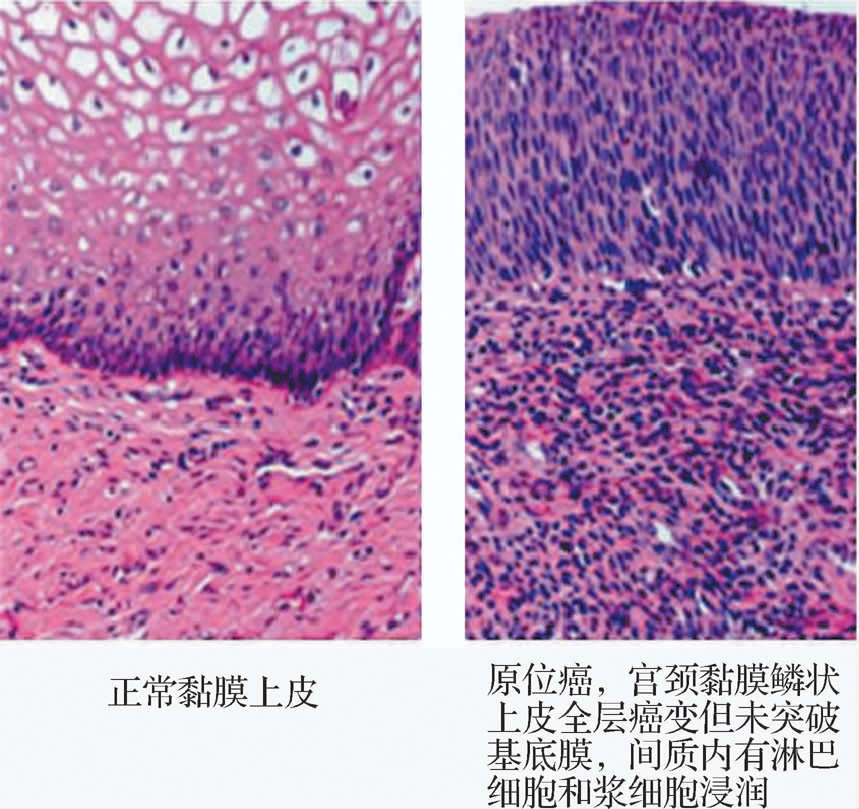
\includegraphics{./images/Image00185.jpg}
 \captionsetup{justification=centering}
 \caption{子宫颈原位癌}
 \label{fig11-1}
  \end{figure} 

\begin{figure}[!htbp]
 \centering
 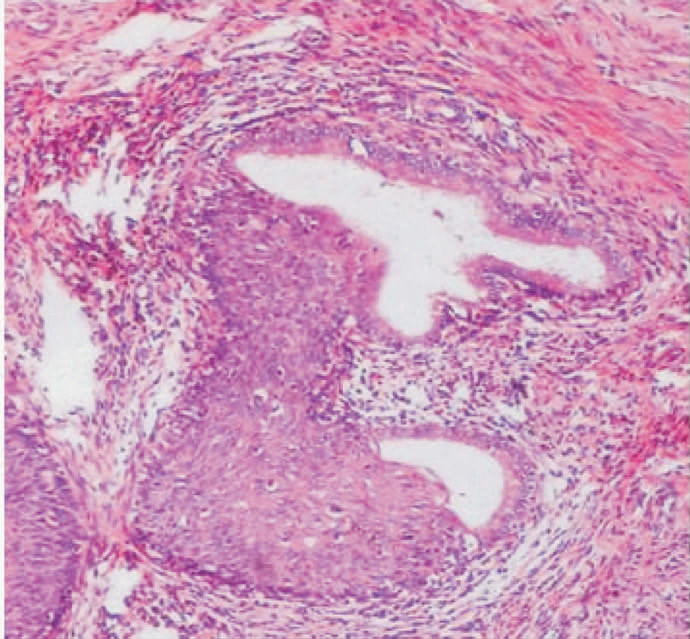
\includegraphics{./images/Image00186.jpg}
 \captionsetup{justification=centering}
 \caption{子宫颈原位癌累及腺体(HE染色,低倍)\\{\small 宫颈原位癌的癌细胞沿基膜通过宫颈腺口蔓延至子宫颈腺体内,取代部分腺上皮}}
 \label{fig11-2}
  \end{figure} 

从鳞状上皮非典型增生到原位癌呈一逐渐演化的级谱样变化,而不是相互分离的病变,重度非典型增生和原位癌的鉴别诊断有一定困难,二者的生物学行为亦无显著的差异。为了解决这些问题,新近的分类将子宫颈上皮非典型增生和原位癌称为子宫颈上皮内瘤变(cervical
intraepithelial
neoplasia,CIN),CINⅠ相当于非典型增生Ⅰ级,属低级别上皮内肿瘤;CINⅡ相当于非典型增生Ⅱ级;CIN
Ⅲ包括非典型增生Ⅲ级和原位癌,CINⅡ和CIN Ⅲ属高级别上皮内肿瘤。

子宫颈上皮CINⅠ和CIN Ⅱ并不一定都发展为CIN
Ⅲ和浸润癌,如经适当治疗,大多数CIN可逆转或治愈。发展为CIN
Ⅲ和浸润癌的几率和所需时间与上皮内瘤变的程度有关。

子宫颈上皮CIN大多无自觉症状,肉眼上与慢性宫颈炎、宫颈糜烂无法加以区别,只能通过细胞学检查才能加以确定。然而临床上可采用碘溶液涂抹加以鉴别,正常宫颈上皮富含糖原,故对碘液着色,如患处对碘液不着色,提示有病变。

\paragraph{子宫颈浸润癌}
宫颈癌的组织发生来源于宫颈阴道部或移行带的鳞状上皮、柱状上皮下的储备细胞及子宫颈管黏膜柱状上皮。

肉眼观分为三型:

(1)外生菜花型:最常见,癌组织主要向子宫颈表面生长,呈灰白或淡粉红色乳头状或菜花状,触之易脱落,因继发感染和肿瘤坏死,常伴有稀薄黄色恶臭液形成。

(2)溃疡型:此型较少见,多因肿瘤中心部位发生坏死脱落所致。病变严重时,因坏死组织大量脱落,可形成火山喷口状缺口或溃疡。一旦坏死物阻塞子宫颈管合并感染可致子宫颈管内积脓。

(3)内生浸润型:最少见,肿瘤以内生性生长为主,浸润子宫颈管壁。

宫颈癌在光镜下可分为鳞状细胞癌和腺癌,以鳞癌占绝大多数(90%以上)。

(1)子宫颈鳞状细胞癌(squamous cell carcinoma of the
cervix):几乎所有的子宫颈浸润性鳞状细胞癌都由子宫颈上皮内瘤变(CIN)发展而来,其演变呈一连续发展的过程,即上皮非典型增生------原位癌------浸润癌。

1)早期浸润癌或微小浸润性鳞状细胞癌:是指癌细胞突破基底膜,向间质内浸润,但浸润深度不超过基底膜下5
mm者。早期浸润癌一般肉眼不能判断,只有在显微镜下才能确诊。早期浸润癌很少发生淋巴结转移。

2)浸润癌:是指癌组织向间质内浸润性生长,浸润深度已超过基底膜下5mm者。肿瘤细胞排列成巢状、带状。光镜下可按其细胞分化程度分为高、中、低三级。分化高者可见角化珠和细胞间桥,低分化者细胞异型性大,细胞体积小,呈圆形或梭形似基底细胞,无角化珠和细胞间桥形成,中等分化者则介于上述两种类型之间(图\ref{fig11-3})。

\begin{figure}[!htbp]
 \centering
 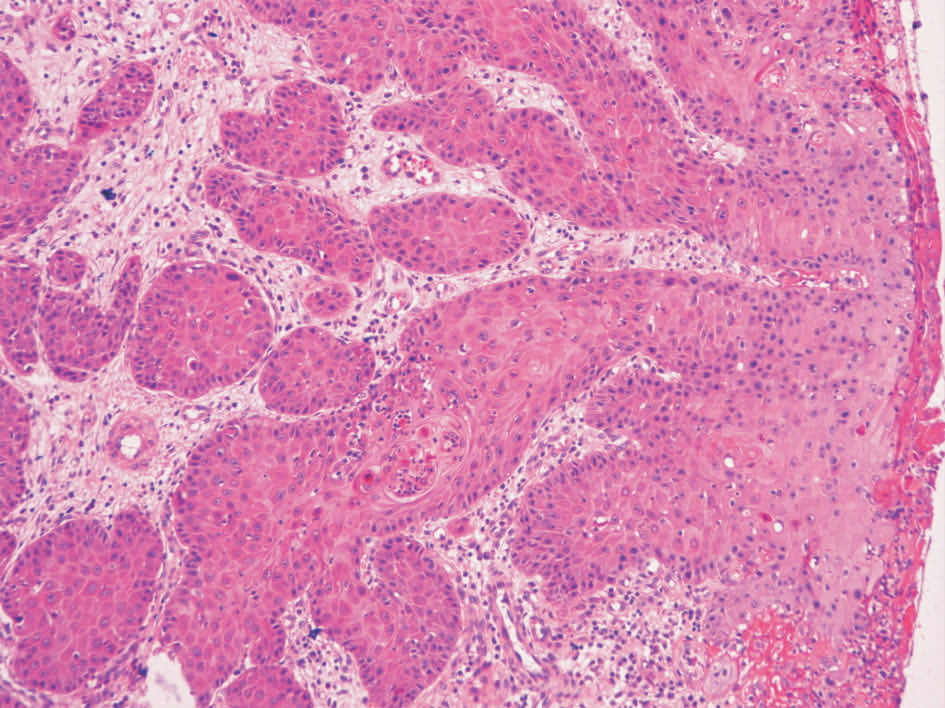
\includegraphics{./images/Image00187.jpg}
 \captionsetup{justification=centering}
 \caption{子宫颈中分化鳞癌(HE染色,低倍)\\ {\small 癌巢浸润至子宫间质,肿瘤细胞排列呈巢状,但无癌珠形成}}
\label{fig11-3}
  \end{figure}

(2)子宫颈腺癌:子宫颈腺癌较鳞癌少见,近年来其发病率有上升趋势,占子宫颈癌的10%~25%。

子宫颈腺癌的病因一般与慢性宫颈炎无关,可能和雌、孕激素失调有关。发病部位可在宫颈外口,或宫颈管内部,宫颈内膜柱状上皮和宫颈黏液腺上皮,少数来自副中肾管残留。腺癌的肉眼形态与鳞癌相似,但镜下呈一般腺癌结构,有时癌细胞具有黏液分泌空泡。个别病例同时伴有腺癌、鳞癌两种成分时,称为腺鳞癌。宫颈腺癌对放疗、化疗的敏感性较低,预后较差。

\subsubsection{扩散}

\paragraph{直接蔓延}
向上浸润破坏整个宫颈段,但很少侵犯子宫体;向下浸润至阴道穹隆及阴道壁;向前侵及膀胱,引起膀胱阴道瘘;向后侵及直肠,引起直肠阴道瘘;向两侧侵及子宫旁及盆腔组织直至骨盆壁。

\paragraph{淋巴道转移}
是子宫颈癌最常见和最重要的转移途径。癌组织首先转移到子宫旁淋巴结,然后依次转移到闭孔、髂外、髂总等盆腔淋巴结。

\paragraph{血道转移}
少见,晚期可经血道转移至肺、骨和肝。

\subsubsection{临床病理联系}

早期子宫颈癌常无自觉症状,与子宫颈糜烂不易区别。随病变进展,因癌组织破坏血管,患者出现不规则阴道流血及接触性出血。因癌组织坏死继发感染,同时由于癌组织刺激宫颈腺体分泌亢进,使白带增多,有特殊腥臭味。晚期因癌组织浸润盆腔神经,可出现下腹部及腰骶部疼痛。当癌组织侵及膀胱及直肠时,可引起尿路阻塞,子宫膀胱瘘或子宫直肠瘘。子宫颈癌死亡原因多见于癌组织坏死引起的大出血和继发性感染所致的败血症或死于双侧输尿管被侵犯阻塞所致的尿毒症。

\section{妊娠滋养层细胞疾病}

绒毛是胎盘的组成单位,表面主要由滋养层上皮的两种细胞,即细胞滋养层细胞和合体滋养层细胞覆盖,具有吸收营养和生成激素(如人绒毛膜促性腺激素,HCG)的功能。绒毛间质内的血管是连接母体和胎儿血液循环的桥梁,因此胎盘异常以及绒毛滋养层细胞病变不仅影响胎儿,而且也可影响母体。本节着重介绍发生在滋养层上皮的三种常见肿瘤,即葡萄胎、侵袭性葡萄胎和绒毛膜上皮细胞癌。其共同特征为滋养层细胞大量增生,患者血清和尿液中HCG含量高于正常妊娠,可作为临床诊断随访观察和评价疗效的辅助指标。

\subsection{葡萄胎}

葡萄胎(hydatidiform
mole)又称水泡状胎块,是胎盘绒毛的一种良性病变,可发生于育龄期的任何年龄,以20岁以下和40岁以上的孕妇中多见,这可能与卵巢功能不足或衰退有关。本病发生有明显地域性差别,欧美国家的发病率约1/2
000,而东南亚地区的发病率比欧美国家高出10倍左右。在我国较为常见,调查统计表明发病率为1/150。

\subsubsection{病因和发病机制}

病因不明。近年来又将葡萄胎分为完全性和部分性两种亚型,根据葡萄胎染色体研究表明,80%以上完全性葡萄胎为46XX,可能在受精时,父方的单倍体精子23X在丢失了所有的母方染色体的空卵中自我复制而成纯合子46XX,两组染色体均来自于父方,缺乏母方功能性DNA;或两个携带有X染色体的单倍体精子在一空卵中结合。其余10%的完全性为空卵在受精时和两个精子结合(23X和23Y),染色体核型为46XY,由于缺乏卵细胞的染色体,故胚胎不能发育,全部绒毛水泡化。

部分性葡萄胎的核型绝大多数为三倍体69XXX或69XXY。由带有母方染色体的正常卵细胞(23X)和一个没有发生减数分裂的双倍体精子(46XY)或两个单倍体精子(23X和23Y)结合所致。可含胚胎成分,仍保留部分正常绒毛。

\subsubsection{病理变化}

肉眼观:病变局限于宫腔内,不侵入肌层。胎盘绒毛高度水肿,形成无数大小不一的水泡,形如葡萄,壁薄而呈透明或半透明状,水泡间有纤细的结缔组织索相连(图\ref{fig11-4})。

\begin{figure}[!htbp]
 \centering
 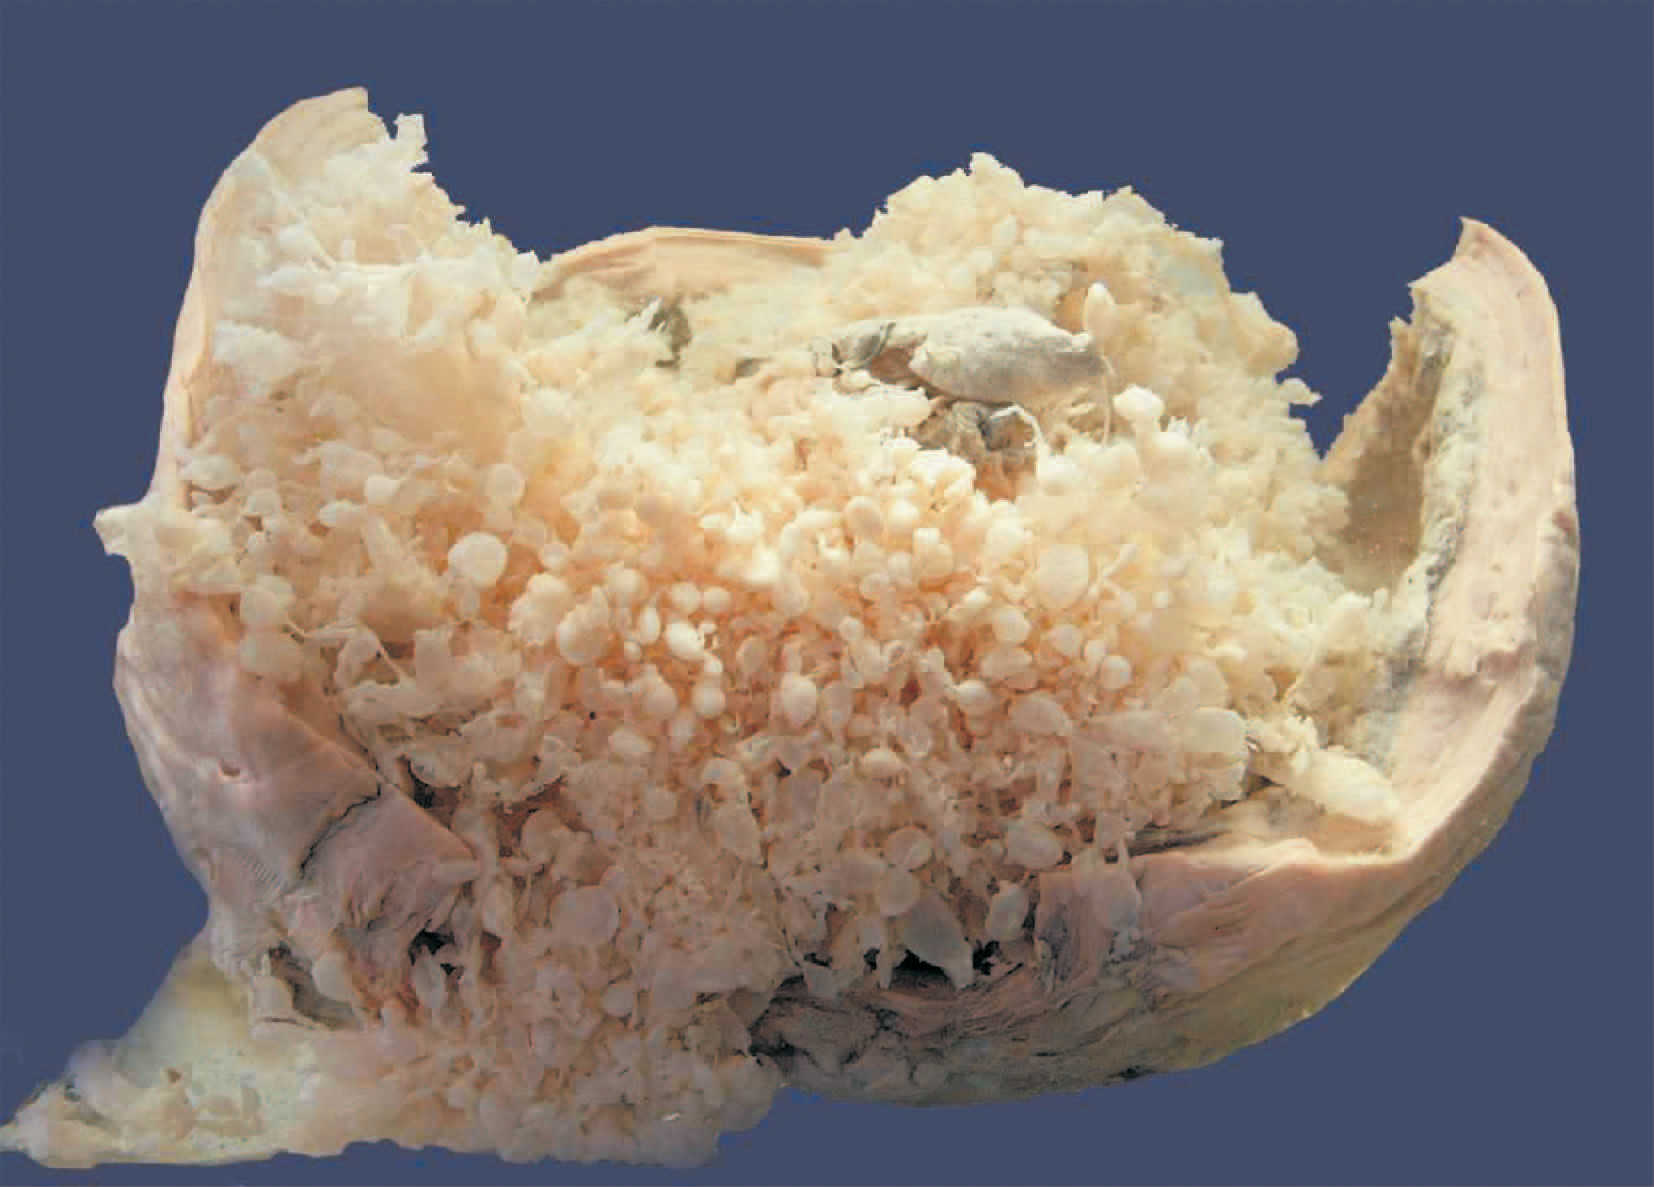
\includegraphics{./images/Image00188.jpg}
 \captionsetup{justification=centering}
 \caption{葡萄胎\\ {\small 子宫已剖开,宫腔内充满水泡样肿物}}
\label{fig11-4}
  \end{figure}

镜下观:葡萄胎有三个特征:①绒毛因间质高度水肿而肿大。②绒毛间质内血管消失,或见少量无功能的毛细血管,内无红细胞。③绒毛滋养层细胞有不同程度增生,增生的细胞包括细胞滋养层细胞和合体滋养层细胞,两者以不同的比例混合存在,并有轻度异型性。滋养层细胞增生为葡萄胎最重要的特征(图\ref{fig11-5})。

\begin{figure}[!htbp]
 \centering
 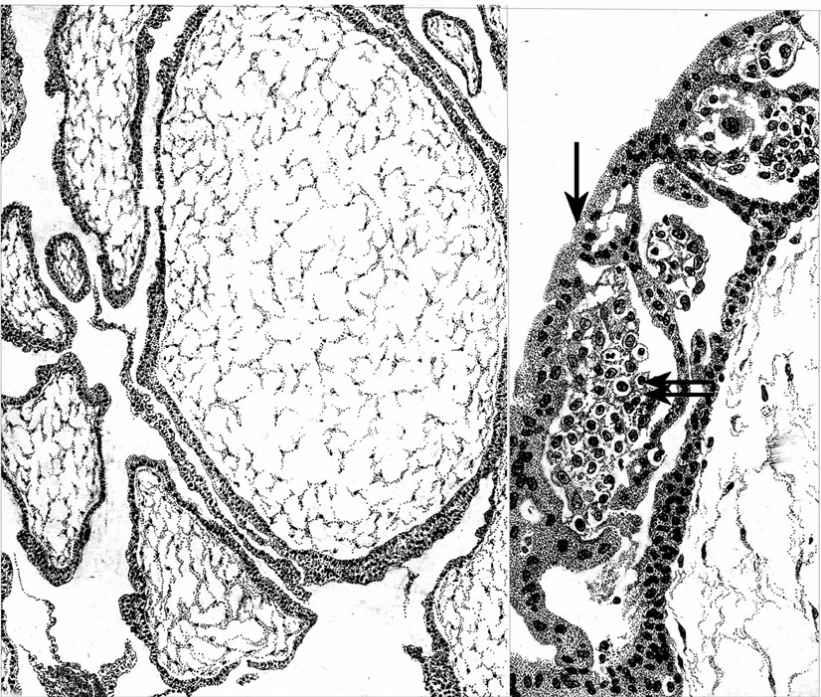
\includegraphics{./images/Image00189.jpg}
 \captionsetup{justification=centering}
 \caption{葡萄胎\\ {\small 左(低倍):绒毛因间质高度水肿,血管消失,局部滋养细胞增生;右(高倍):增生的滋养细胞,其中↓为合体滋养层细胞,$\leftarrow$为细胞滋养层细胞}}
\label{fig11-5}
  \end{figure}

\subsubsection{临床病理联系}

患者多半在妊娠的第12周至14周出现症状,由于胎盘绒毛高度水肿致子宫体明显增大,常超过相同月份正常妊娠的子宫,因胚胎早期死亡,虽然子宫超过5个月妊娠大小,但仍听不到胎心,且无胎动。患者血和尿中绒毛膜促性腺激素(HCG)明显增高。滋养层细胞侵袭血管的能力很强,故子宫反复不规则流血。

葡萄胎经彻底刮宫后,绝大多数可痊愈。约有10%的患者发展为侵袭性葡萄胎,约2.5%病例可发展为绒癌。

\subsection{侵袭性葡萄胎}

侵袭性葡萄胎(invasive mole)又称恶性葡萄胎(malignant
mole),是介于葡萄胎与绒毛膜上皮癌之间的交界性肿瘤。侵袭性葡萄胎和良性葡萄胎的主要区别是在于水泡状绒毛侵入子宫肌层,引起子宫肌层出血坏死,甚至可穿透子宫壁,累及阔韧带和阴道(图\ref{fig11-6})。少数情况下亦可发生肺、脑等内脏的栓塞,但一般不形成转移灶,相反,它常可发生自发性消退。

\begin{figure}[!htbp]
 \centering
 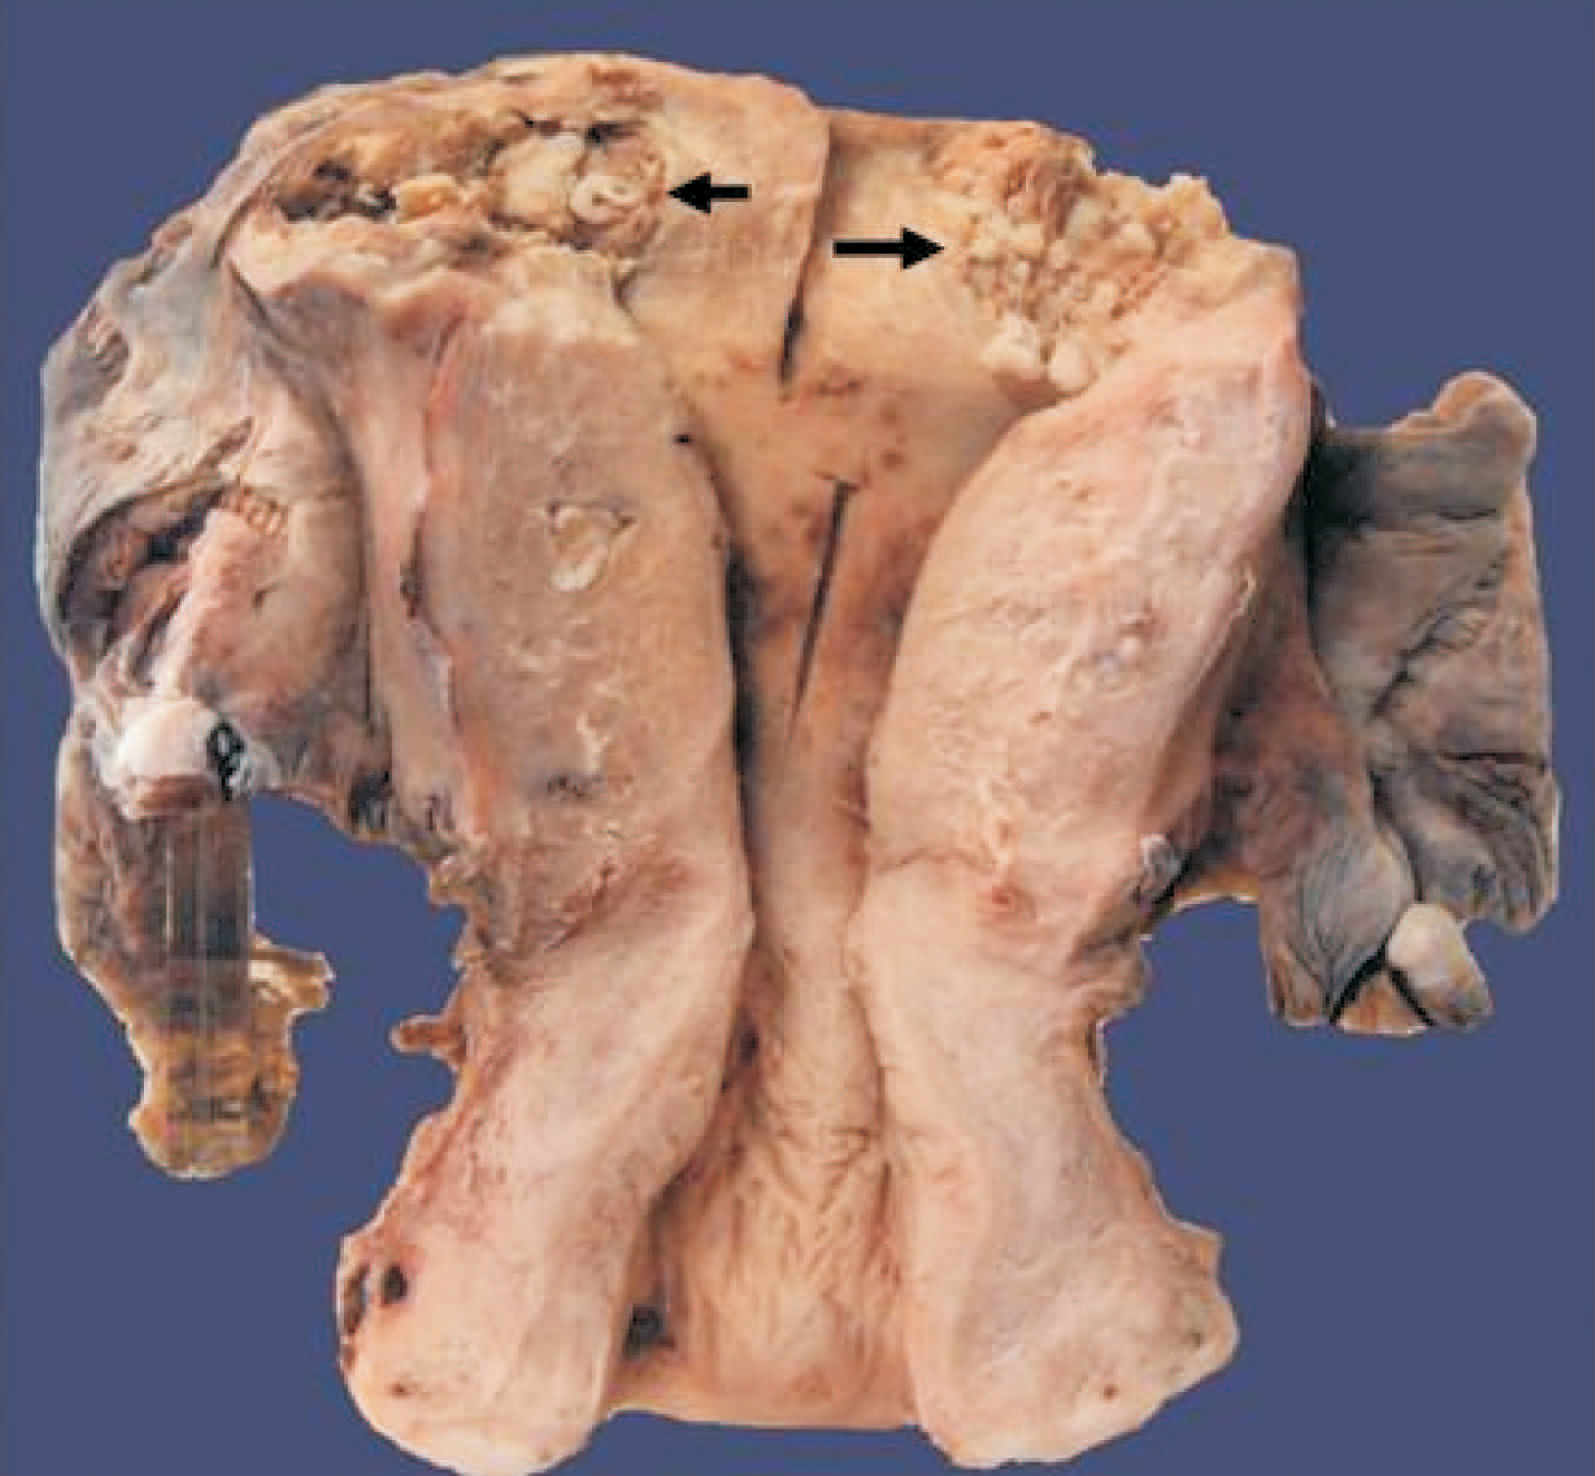
\includegraphics{./images/Image00191.jpg}
 \captionsetup{justification=centering}
 \caption{侵袭性葡萄胎\\ {\small 子宫已破开,宫腔内无水泡样肿物,宫底肌壁中有水泡状绒毛侵入}}
\label{fig11-6}
  \end{figure}

镜下观:滋养层细胞增生的程度和异型性比良性葡萄胎显著。常见出血坏死,其中可查见水泡状绒毛或坏死的绒毛(图\ref{fig11-7}),有无绒毛结构是本病与绒毛膜上皮癌的主要区别。临床主要表现是血和尿中HCG持续阳性,由于恶性葡萄胎具有较强的侵袭性,可侵犯和破坏血管和血窦,导致患者在水泡状胎块清宫后,出现持续、不规则的阴道流血,化疗对大多数病例治疗有效。

\begin{figure}[!htbp]
 \centering
 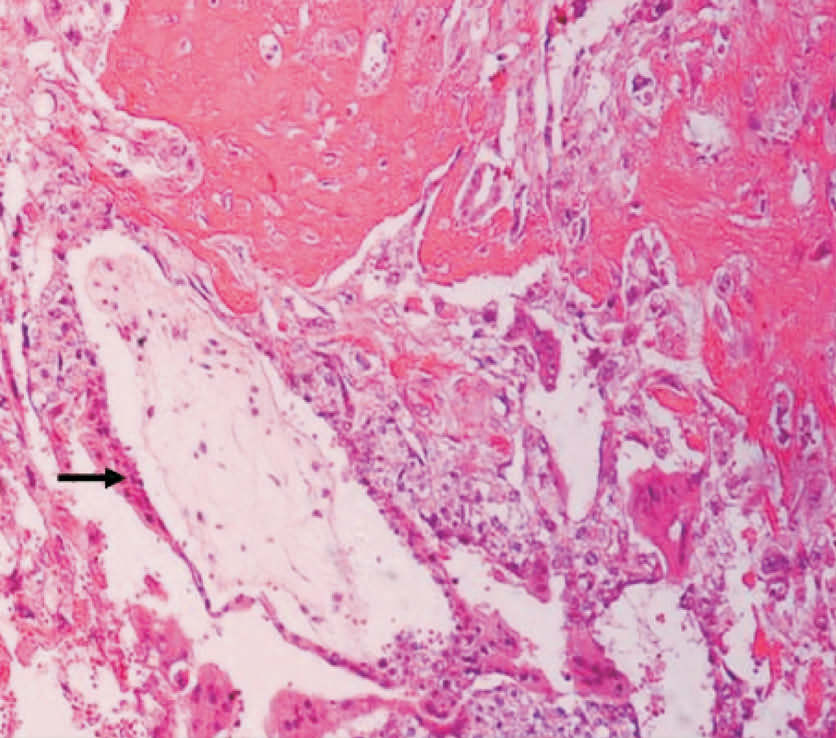
\includegraphics{./images/Image00192.jpg}
 \captionsetup{justification=centering}
 \caption{侵袭性葡萄胎\\ {\small 异常增生的滋养层细胞侵及子宫肌层,仍可见绒毛结构(箭头示)(HE染色,低倍)}}
\label{fig11-7}
  \end{figure}

\subsection{绒毛膜上皮癌}

绒毛膜上皮癌(choriocarcinoma)简称绒癌,是一种高度恶性的滋养层细胞肿瘤,其发生绝大多数与妊娠有关,约50%的病例来自葡萄胎,尤以完全性葡萄胎为常见;约25%来自流产,其余大多数则来自正常妊娠。罕见的情况下绒癌发生与妊娠无关,起源于性腺或其他部位的全能性细胞,此时的绒癌为生殖细胞肿瘤,男女两性均可发生。

\subsubsection{病理变化}

肉眼观:肿瘤为单个或多个结节,呈暗红色、质脆,多数突向宫腔内,大小不一,少数肿瘤则以浸润性生长方式为主,并可穿破子宫肌层达浆膜、子宫旁或侵入盆腔,形成不规则出血性肿块(图\ref{fig11-8})。

\begin{figure}[!htbp]
 \centering
 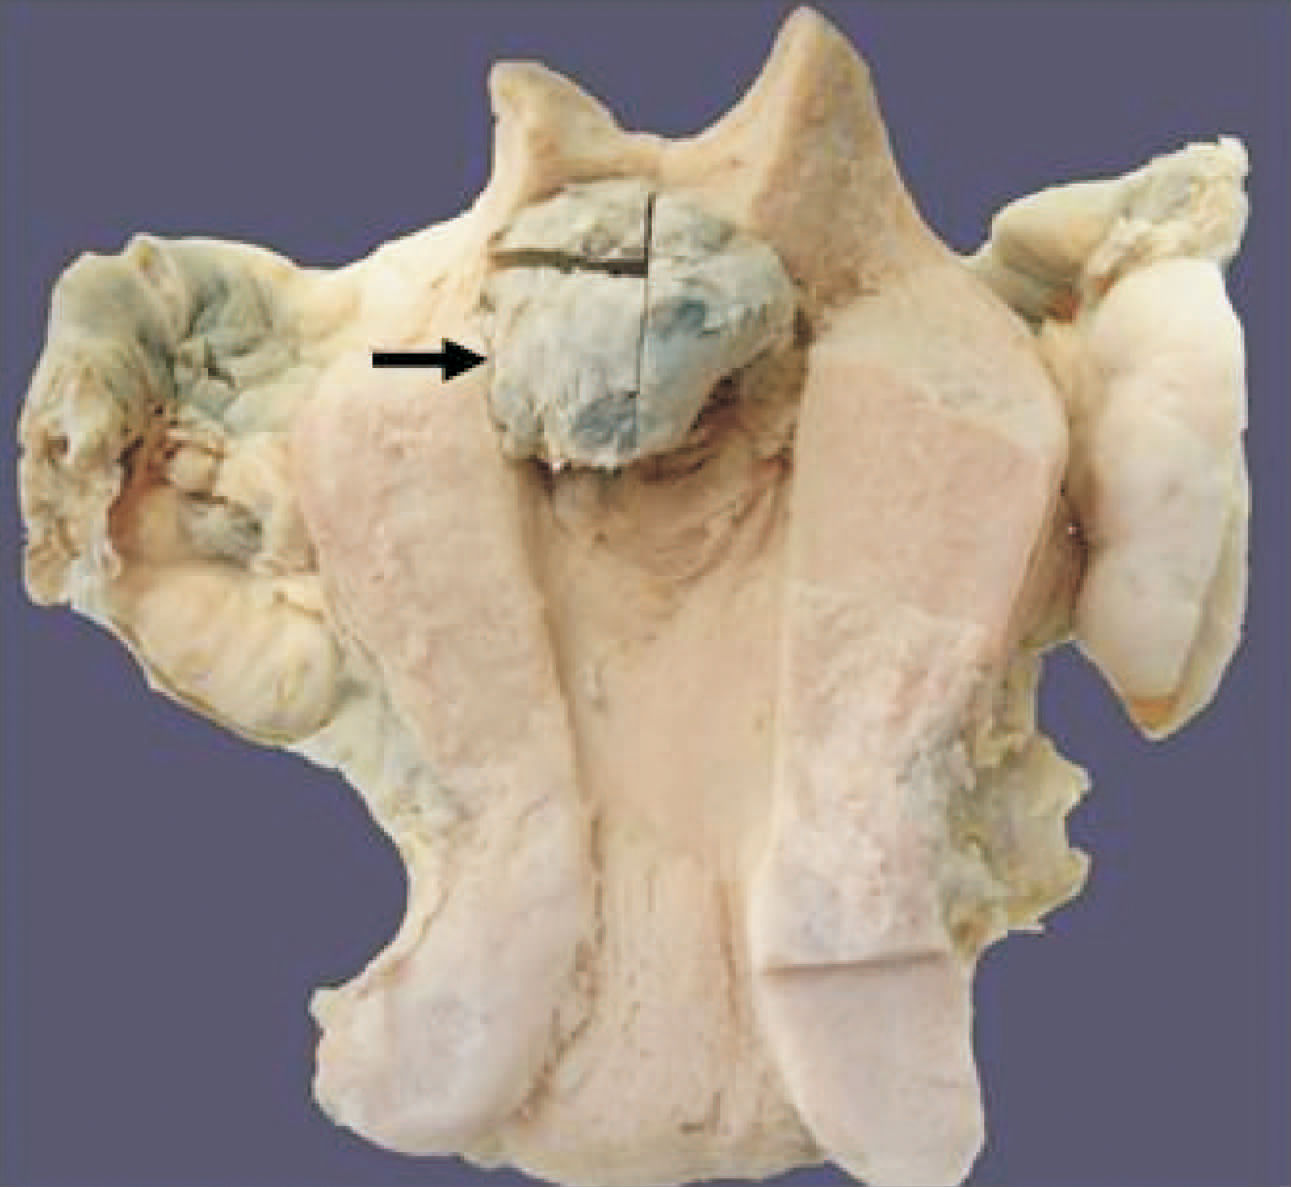
\includegraphics{./images/Image00193.jpg}
 \captionsetup{justification=centering}
 \caption{绒毛膜上皮细胞癌\\ {\small 子宫已破开,癌组织形成结节状出血块}}
\label{fig11-8}
  \end{figure}

镜下:①癌组织由异常增生的细胞滋养层细胞和合体滋养层细胞组成,两种癌细胞多少不等,排列紊乱,参差相嵌组成团状或条索状癌细胞巢,但不伴有间质和血管。②出血坏死明显,此乃肿瘤缺乏血管而靠侵袭邻近血管获取营养、且生长迅速而发生缺血性坏死所致;③无绒毛或水泡形成(图\ref{fig11-9})。

\begin{figure}[!htbp]
 \centering
 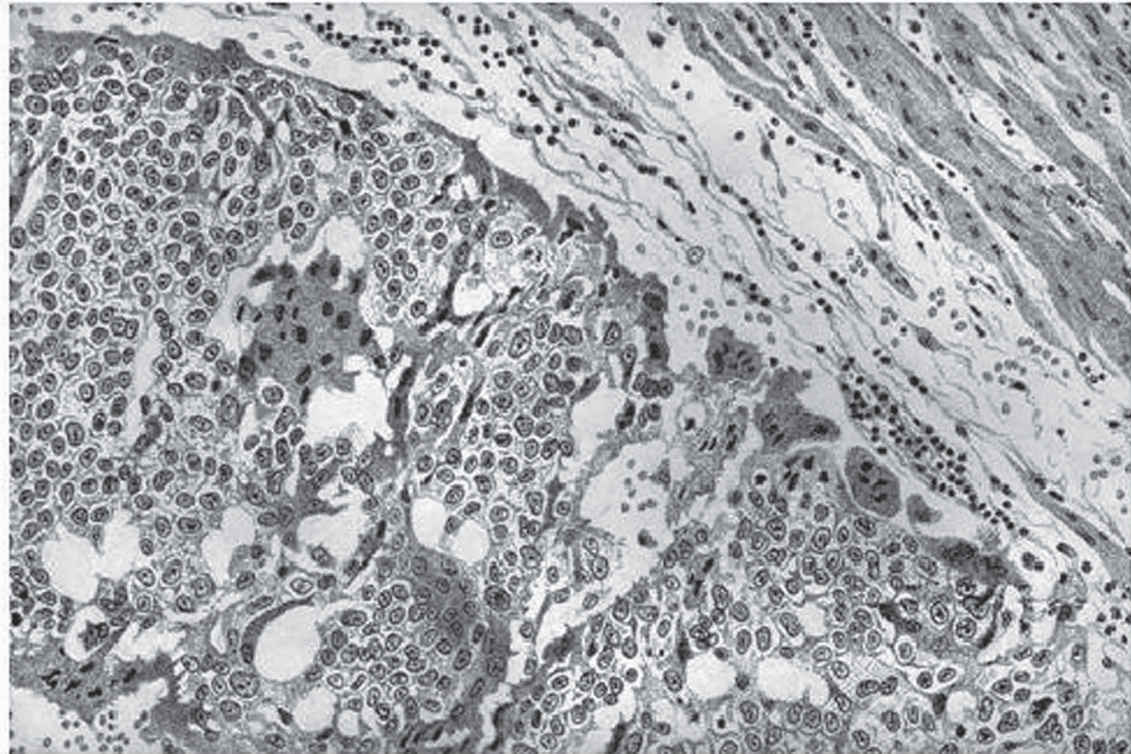
\includegraphics{./images/Image00194.jpg}
 \captionsetup{justification=centering}
 \caption{绒毛膜上皮细胞癌\\ {\small 子宫肌层内大量肿瘤细胞浸润,癌细胞由两种滋养层细胞构成,有明显的异型性,不形成绒毛结构}}
\label{fig11-9}
  \end{figure}

\subsubsection{扩散}

绒癌侵袭破坏血管的能力很强,除在局部破坏蔓延外,极易经血道转移,以肺和阴道壁最常见,其次为脑、肝、肾、脾等,转移灶呈球形出血性结节,少数病例在切除原发病灶后,转移灶自行消失。

\subsubsection{临床病理联系}

绒癌主要症状为阴道大量不规则流血,子宫增大迅速,血和尿内有高滴度的HCG,但有时也可转为阴性,可能因为肿瘤坏死明显,存活的滋养层细胞减少之故。所以产后或流产后特别是葡萄胎患者血、尿中HCG时高时低,或持续升高,应考虑绒癌的可能。一旦肿瘤发生远处转移,则可引起转移部位的症状,如肺转移可发生咯血,胸膜转移出现血性胸水,脑转移则可出现抽搐、瘫痪或昏迷等。

绒癌是恶性度很高的肿瘤,以往治疗以手术为主,多在一年内死亡。近年来通过化疗,其死亡率大为降低,治愈率已接近100%,甚至治愈后可正常妊娠。

\begin{table}[ht]
    \caption{葡萄胎、侵袭性葡萄胎、绒毛膜癌比较}
    \label{tab11-1}
    \centering
    \begin{tabular}{cccc}
    \toprule
    &葡萄胎&侵袭性葡萄胎&绒毛膜上皮癌\\
    \midrule
    组织起源&滋养层细胞&滋养层细胞&滋养层细胞\\
良恶性&良性&恶性&恶性\\
绒毛结构&有&有&无\\
滋养层细胞增生&2+&3+&4+\\
出血坏死&无&可有&显著\\
血、尿HCG&增高&增高&增高\\
局部浸润&无&有&有\\
转移&无&有&有\\
    \bottomrule
    \end{tabular}
\end{table}

\section{卵巢肿瘤}

卵巢肿瘤种类繁多,结构复杂,依照其组织发生可分为三大类。

\paragraph{上皮性肿瘤}
浆液性肿瘤、黏液性肿瘤、子宫内膜样肿瘤、透明细胞肿瘤及移行细胞肿瘤。

\paragraph{性索间质肿瘤}
颗粒细胞-卵泡膜细胞瘤、支持-间质细胞瘤。

\paragraph{生殖细胞肿瘤}
畸胎瘤、无性细胞瘤、内胚窦瘤及绒毛膜癌。

卵巢肿瘤多见于20~65岁的女性,其中恶性上皮性恶性肿瘤多发生于40岁以后。卵巢癌的病因至今尚不明确,不育和不哺乳、排卵因素、外用雌激素、电离辐射等因素被认为是高危因素,BRCA1基因被证实在卵巢癌发生中起重要作用。

\subsection{卵巢表面上皮-间质性肿瘤}

卵巢上皮性肿瘤是最常见的卵巢肿瘤,占所有卵巢肿瘤的90%,可分为良性、恶性和交界性。交界性卵巢上皮性肿瘤是指形态和生物学行为介于良性和恶性之间,具有低度恶性潜能的肿瘤。此类肿瘤主要来源于覆盖在卵巢表面的腹膜间皮细胞,有多少不等的间质参与,形态复杂多样。依据上皮的类型不同分为浆液性、黏液性和子宫内膜样肿瘤。

\subsubsection{浆液性肿瘤}

浆液性囊腺瘤(serious
cystadenoma)是卵巢最常见的肿瘤,其中浆液性囊腺癌占全部卵巢癌的1/3。良性和交界性肿瘤多发于30~40岁的女性,而囊腺癌患者则年龄偏大。

肉眼观,由单个或多个纤维分隔的囊腔组成,囊内含有清亮液体。良性瘤囊内壁光滑,交界性囊腺瘤囊壁可见较多乳头(图\ref{fig11-10}a),大量实性组织和乳头在肿瘤中出现时应疑为癌。

镜下,良性瘤囊腔由单层立方或矮柱状上皮衬覆,上皮细胞排列整齐,乳头间质由纤维脉管构成(图\ref{fig11-10}b)。交界瘤上皮细胞达两至三层,乳头增多,细胞核分裂象增加;新近的研究证明间质浸润灶不超过10
mm的交界性浆液性乳头状囊腺瘤的预后和无间质浸润的交界性浆液性乳头状囊腺瘤的预后相似,称为具有微小浸润的交界性浆液性乳头状囊腺瘤。浆液性囊腺癌细胞层次增加超过三层(图\ref{fig11-10}c),伴有明显的癌细胞破坏性间质浸润,常可见砂粒体。

\begin{figure}[!htbp]
 \centering
 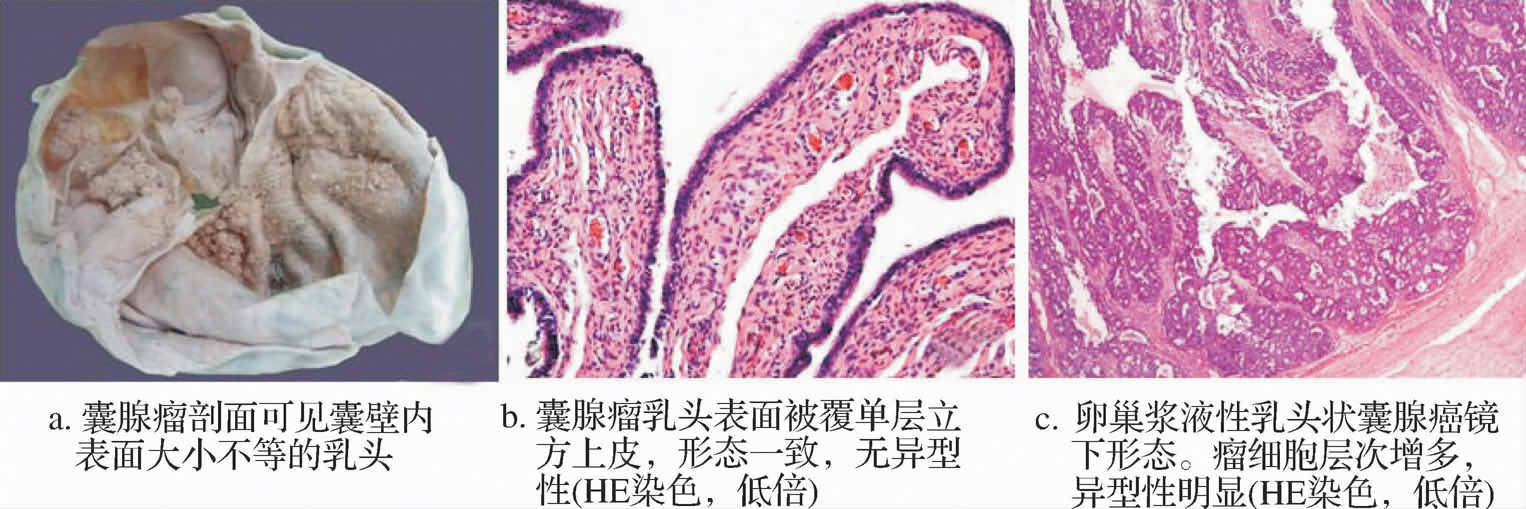
\includegraphics{./images/Image00196.jpg}
 \captionsetup{justification=centering}
 \caption{卵巢浆液性肿瘤}
 \label{fig11-10}
  \end{figure} 

\subsubsection{黏液性肿瘤}

黏液性肿瘤(mucinous
tumors)较浆液性肿瘤少见,多数为良性,交界性和恶性少见。发病年龄与浆液性肿瘤相同。

肉眼观,肿瘤表面光滑,由多个大小不一的囊腔组成,囊壁光滑,腔内充满富于糖蛋白的灰白色半透明黏稠液体(图\ref{fig11-11}a)。

镜下,良性黏液性囊腺瘤的囊腔被覆单层高柱状上皮,核在基底部,核的上部充满黏液,无纤毛(图\ref{fig11-11}b)。交界性肿瘤含有较多的乳头结构,细胞层数不超过3层,但无间质和被膜浸润:囊性癌上皮细胞明显异型,形成复杂的腺体和乳头结构,可有出芽、搭桥及实性巢状区,如有间质明显破坏性浸润,可诊断为癌。

\begin{table}[ht]
    \caption{良性浆液性及黏液性囊腺瘤的区别}
    \label{tab11-2}
    \centering
    \begin{tabular}{ccc}
    \toprule
    &良性浆液性囊腺瘤&良性黏液性囊腺瘤\\
    \midrule
    单房或多房&多为单房&多为多房\\
囊内液体&清亮浆液&黏稠黏液\\
乳头&可有&少见\\
囊壁&低立方状上皮&高柱状黏液上皮\\
恶变&多见&少见\\
    \bottomrule
    \end{tabular}
\end{table}

\begin{figure}[!htbp]
 \centering
 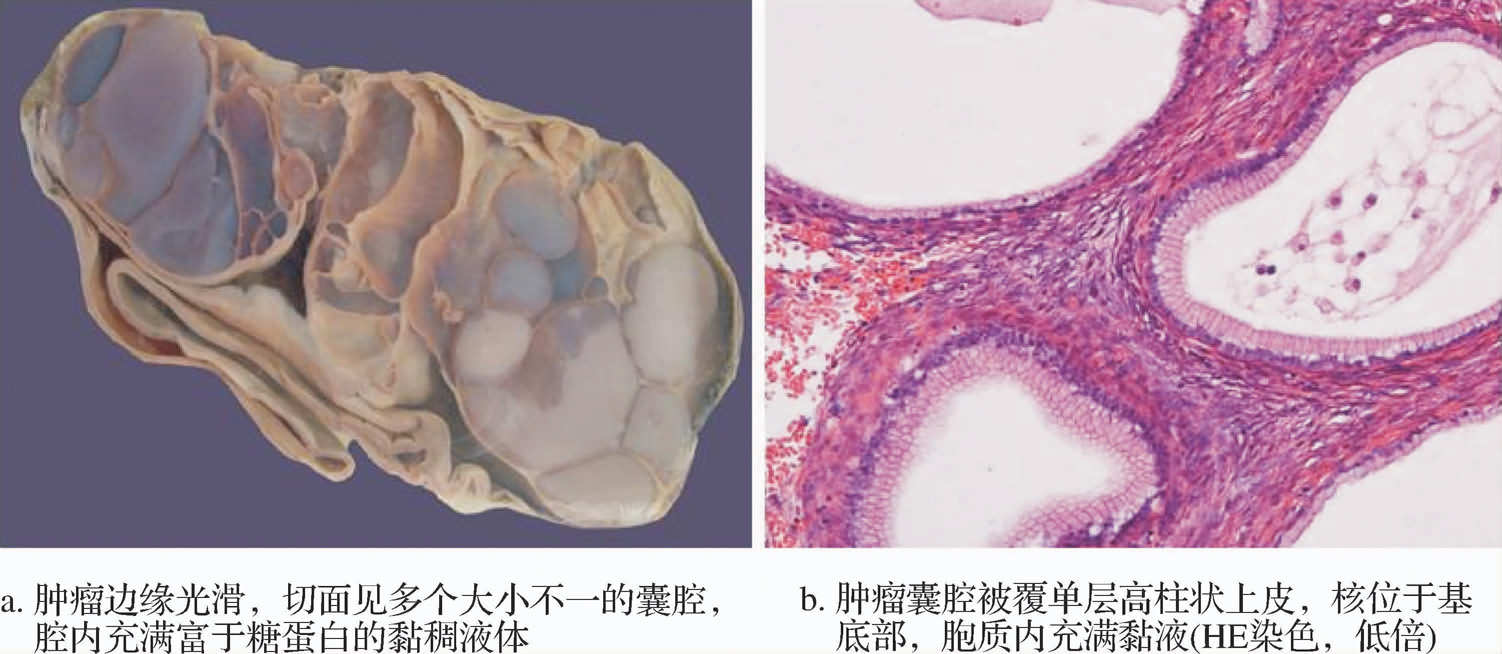
\includegraphics{./images/Image00198.jpg}
 \captionsetup{justification=centering}
 \caption{卵巢黏液性囊腺瘤}
 \label{fig11-11}
  \end{figure} 

\subsection{性索间质肿瘤}

卵巢性索间质肿瘤起源于原始性腺中的性索和间质组织,分别在男性和女性衍化成各自不同类型的细胞,并形成一定的组织结构。包括女性的颗粒细胞瘤和卵泡膜细胞瘤,或男性的支持细胞瘤和间质细胞瘤;亦可混合构成颗粒细胞-卵泡膜细胞瘤或支持-间质细胞瘤。由于性索间质可向多方向分化,卵巢和睾丸可查见所有这些细胞类型来源的肿瘤。卵泡膜细胞和间质细胞可分别产生雌激素和雄激素,患者常有内分泌功能改变。

\subsubsection{颗粒细胞瘤}

颗粒细胞瘤(granulosa cell
tumor)是伴有雌激素分泌的功能性肿瘤。虽然该瘤极少发生转移,但可发生局部扩散,甚至在切除多年后复发,应被看做低度恶性肿瘤。肉眼观,颗粒细胞瘤体积较大,呈囊实性,部分区域呈黄色,常伴发出血。镜下,瘤细胞小而一致,排列成弥漫型、岛屿型或梁索型,细胞核可见核沟,分化较好的瘤细胞常排列成卵泡样的结构,中央为粉染的蛋白液体或退化的细胞核,称为Call-Exner小体。

\subsubsection{卵泡膜细胞瘤}

卵泡膜细胞瘤(thecoma)为良性功能性肿瘤,可产生雌激素,绝大多数患者有雌激素产生增多的体征,患者常表现为月经不调和乳腺增大,多发生于绝经后的妇女。肿瘤呈实体状,色黄,瘤细胞呈束状排列,细胞呈空泡状。

\subsubsection{支持-间质细胞瘤}

支持-间质细胞瘤(sertoli-leydig cell
tumors)主要发生在睾丸,较少发生于卵巢,任何年龄均可发病,多发于年轻育龄期妇女。该瘤可分泌少量雄激素,若大量分泌可表现为男性化。

\subsection{卵巢生殖细胞肿瘤}

来源于生殖细胞的肿瘤约占所有卵巢肿瘤的1/4,好发于青少年女性。多数为恶性,仅畸胎瘤可有良性类型。原始生殖细胞具有向不同方向分化的潜能,由原始性生殖细胞组成的肿瘤称作无性细胞瘤;原始生殖细胞向胚胎的体壁细胞分化称为畸胎瘤;向胚外组织分化,瘤细胞和胎盘的间充质细胞或它的前身相似,称作卵黄囊瘤;向覆盖在胎盘绒毛表面的细胞分化,则称为绒毛膜癌。

\subsubsection{畸胎瘤}

畸胎瘤(teratoma)是来源于生殖细胞的肿瘤,具有向体细胞分化的潜能,大多数肿瘤含有至少两个或三个胚层组织成分。占所有卵巢肿瘤的15%~20%,好发于20~30岁女性。

\paragraph{成熟畸胎瘤}
是最常见的生殖细胞肿瘤。肉眼观,肿瘤多为囊性,呈圆形或椭圆形,切面多为单房,囊内含有皮脂样物、毛发,牙齿等(图\ref{fig11-12})。镜下,肿瘤由两个或三个胚层的各种成熟组织构成。常见皮肤、毛囊、汗腺、脂肪、肌肉、骨、软骨、呼吸道上皮、消化道上皮、甲状腺和脑组织等(图\ref{fig11-13})。1%可发生恶性变,多发生在老年女性。

\begin{figure}[!htbp]
 \centering
 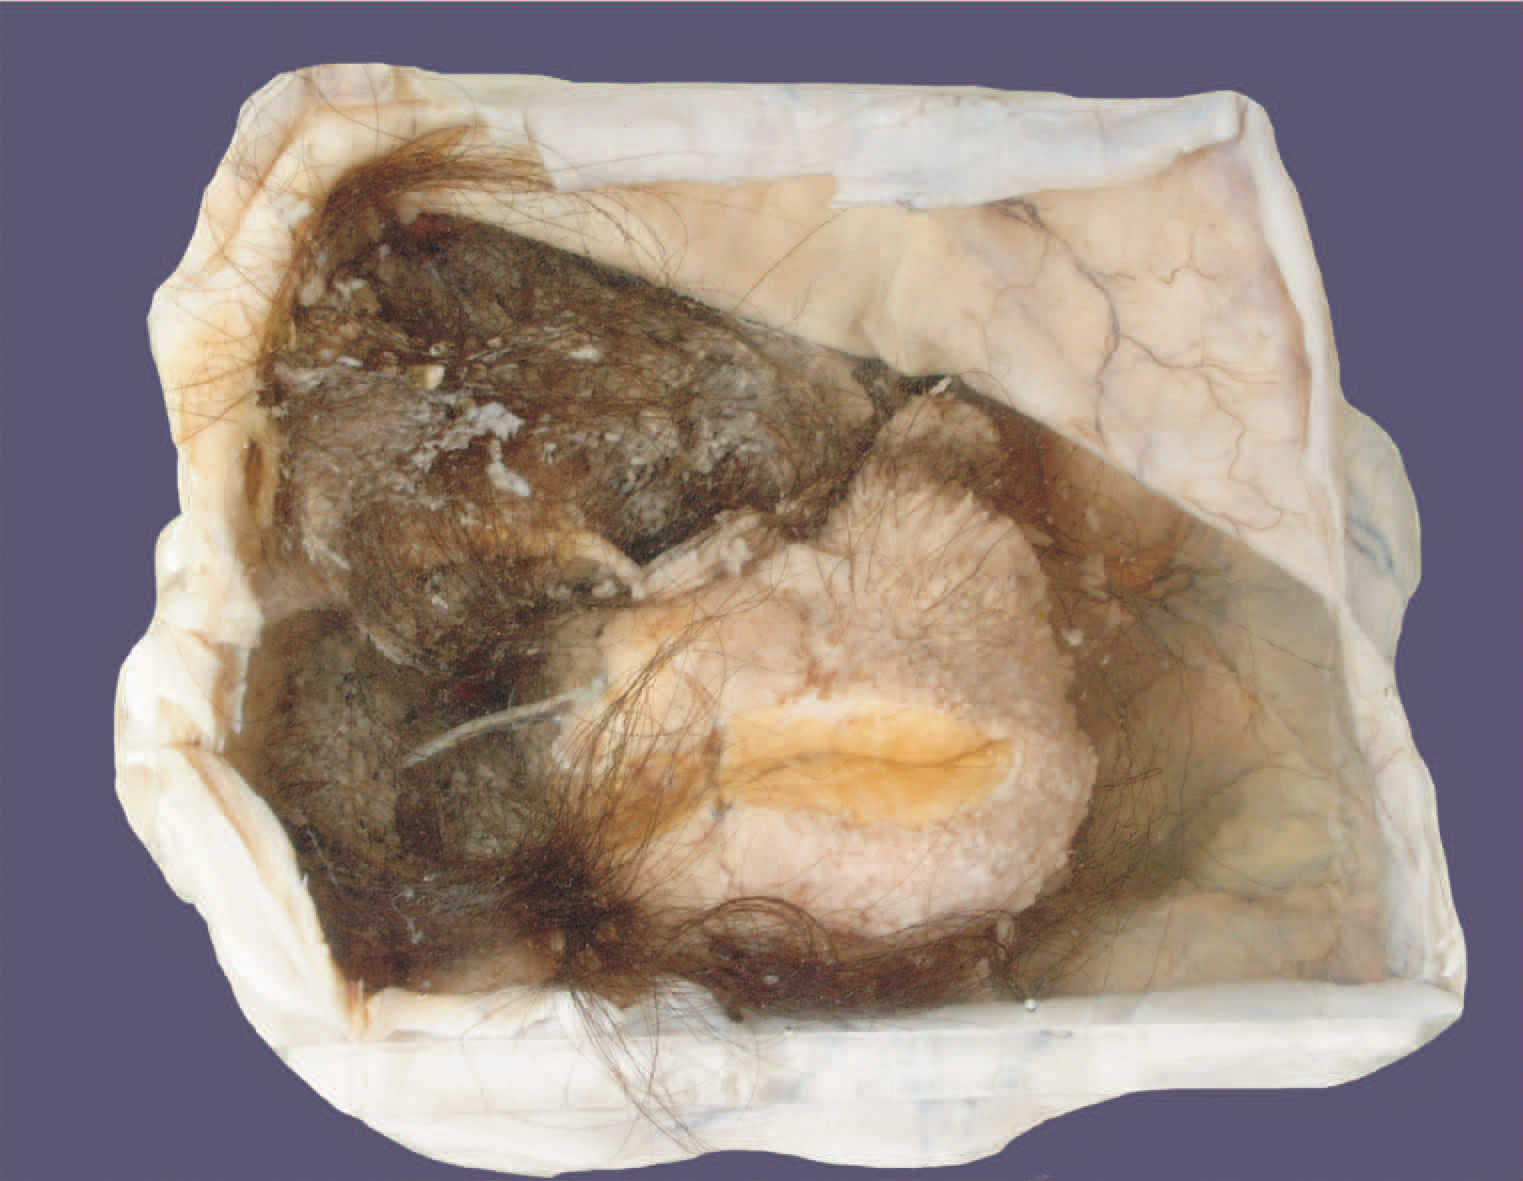
\includegraphics{./images/Image00199.jpg}
 \captionsetup{justification=centering}
 \caption{卵巢成熟性畸胎瘤\\ {\small 肿瘤囊壁内可见毛发、皮脂样物、牙齿}}
\label{fig11-12}
  \end{figure}

\begin{figure}[!htbp]
 \centering
 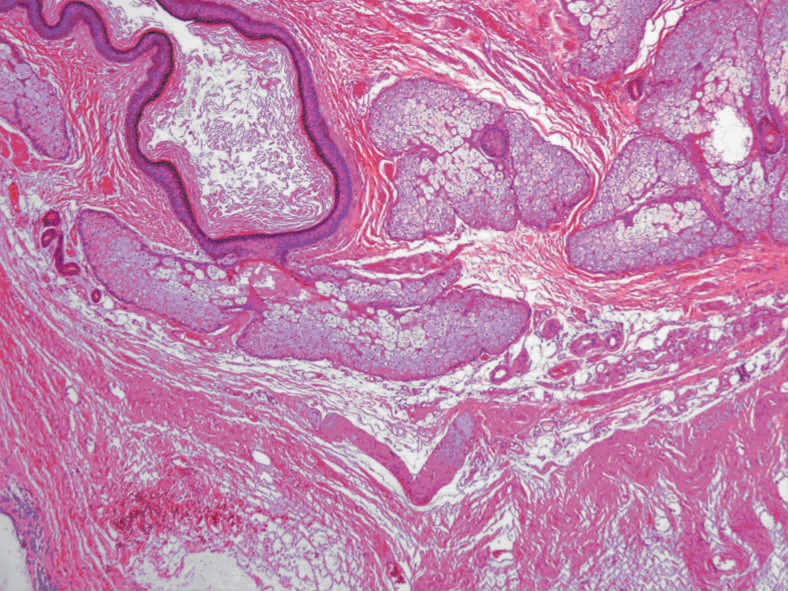
\includegraphics{./images/Image00200.jpg}
 \captionsetup{justification=centering}
 \caption{卵巢成熟性畸胎瘤(HE染色,低倍)\\ {\small 肿瘤成分中可见鳞状上皮、皮脂腺、汗腺及神经组织}}
\label{fig11-13}
  \end{figure}

\paragraph{未成熟性畸胎瘤}
以肿瘤组织中查见未成熟组织为特征,肿瘤多为实体分叶状,可含有多个小的囊腔,预后与肿瘤分化程度有关(图\ref{fig11-14})。

\begin{figure}[!htbp]
 \centering
 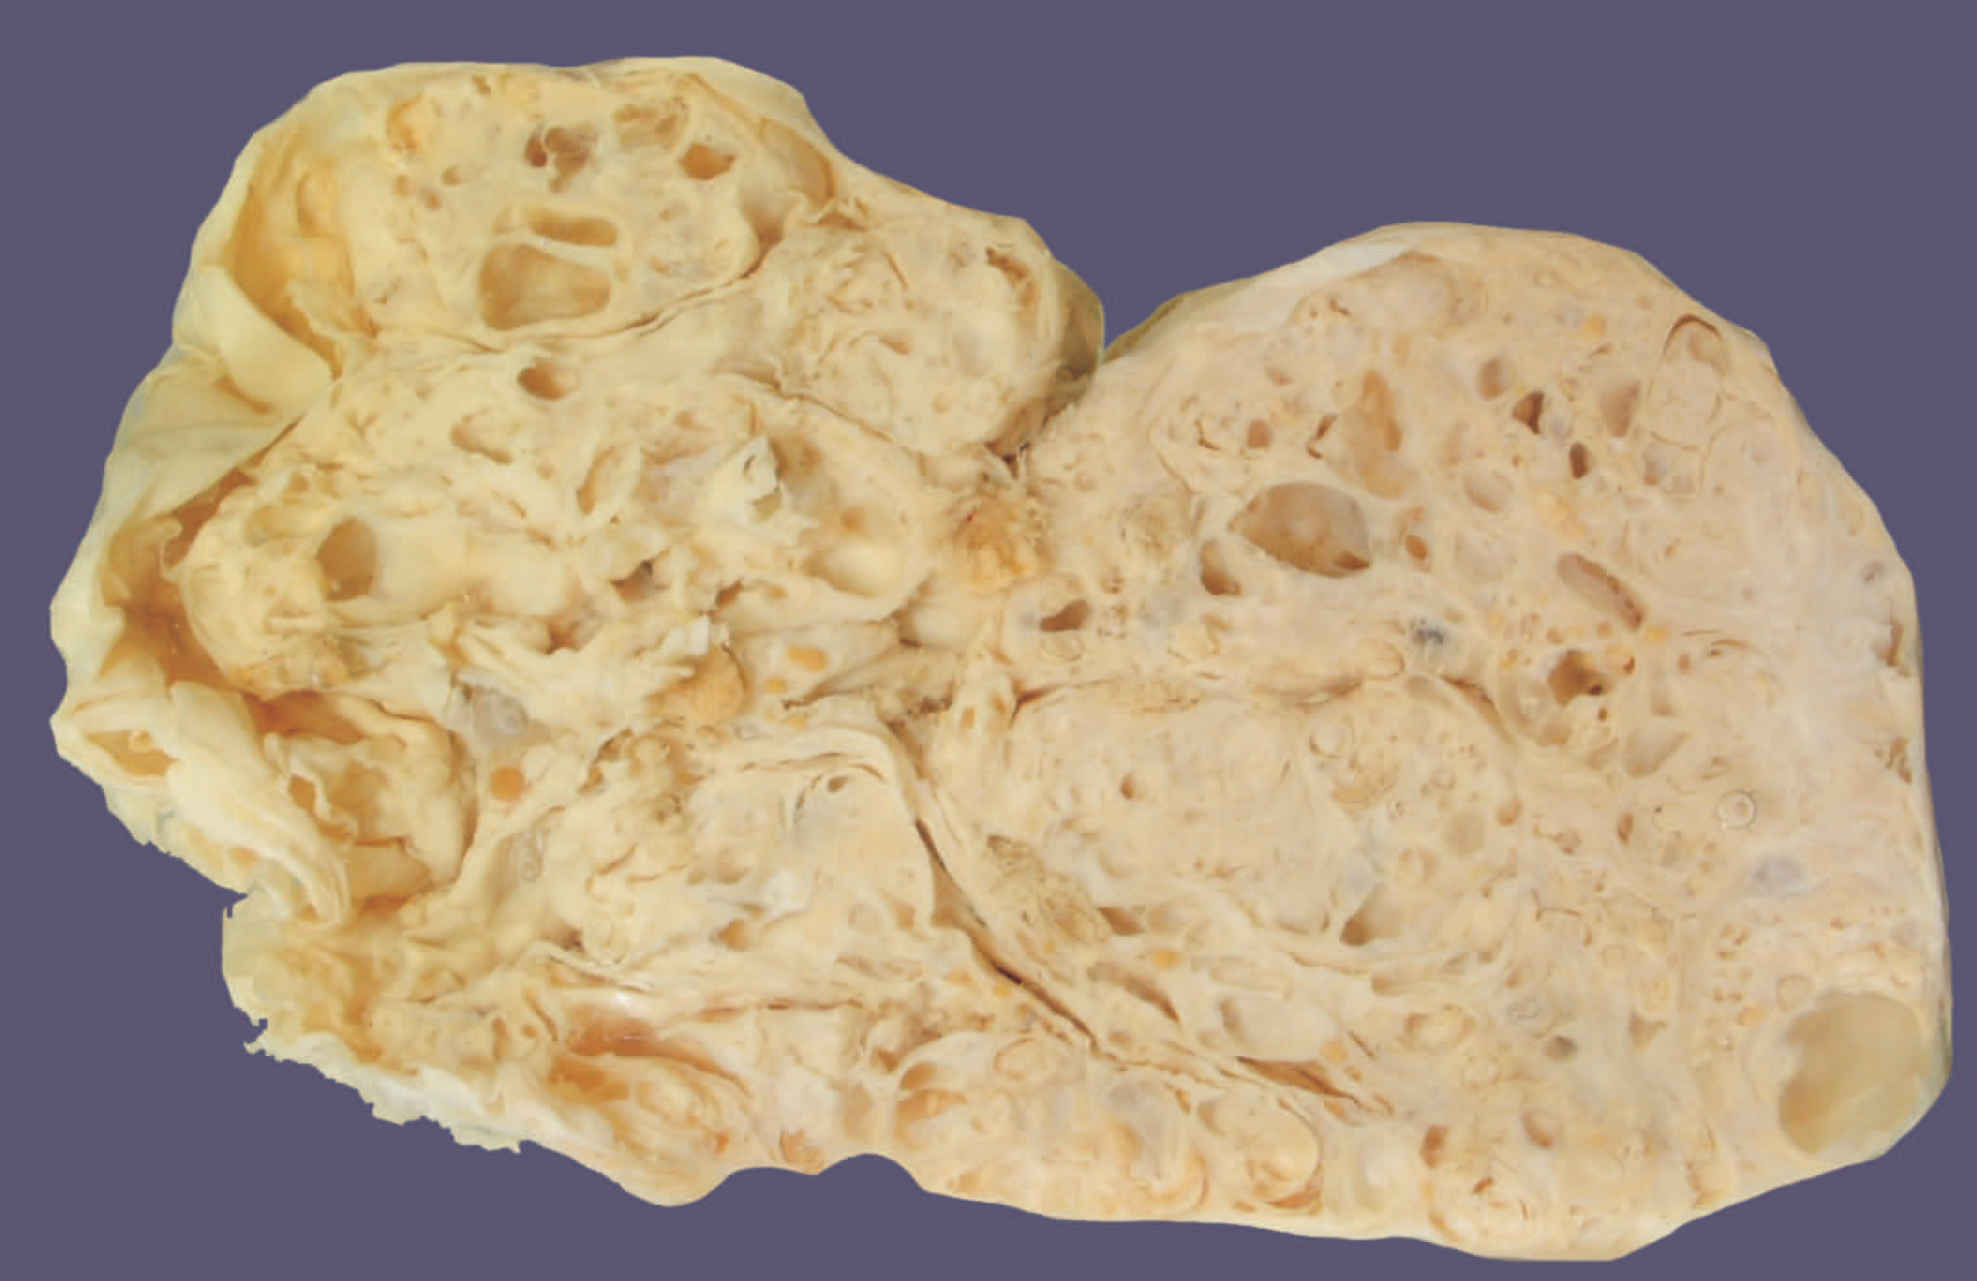
\includegraphics{./images/Image00201.jpg}
 \captionsetup{justification=centering}
 \caption{卵巢未成熟性畸胎瘤\\ {\small 肿瘤呈实体分叶状,内含多个小囊腔}}
\label{fig11-14}
  \end{figure}

\subsubsection{无性细胞瘤}

无性细胞瘤(dysgerminoma)是由未分化、多潜能原始生殖细胞组成的恶性肿瘤,好发年龄在10~30岁。发生在睾丸则称为精原细胞瘤(seminoma),是睾丸最常见的肿瘤。肿瘤一般体积较大,质实,表面结节状,切面质软鱼肉样。镜下,细胞体积大,形态相似,呈圆形或多边形,胞质丰富透明,核分裂象多见。无性细胞瘤对放疗和化疗敏感,5年生存率可达80%以上。晚期主要经淋巴道转移至髂部和主动脉旁淋巴结。

\subsubsection{胚胎性癌}

胚胎性癌(embryonal
carcinoma)主要发生于20~30岁的青年人,是高度恶性的肿瘤。肉眼观,肿瘤体积小,切面肿瘤边界不清,可见出血和坏死。镜下,以癌组织结构多样性为特征,核分裂象较多见;间质形态很不一致。此癌生长迅速,放疗不敏感,转移早,预后差。

\subsubsection{卵黄囊瘤}

卵黄囊瘤(yolk sac
tumor)又称内胚窦瘤,因组织形态和小鼠胎盘的结构很相似而取此名,多发生在30岁以下妇女,是婴幼儿生殖细胞肿瘤中最常见的类型,生物学行为呈高度恶性。肿瘤体积一般较大,结节分叶状,边界不清,切面灰黄色,呈实体状,局部可见囊腔形成和出血坏死。镜下有多种组织形态,可见疏网状结构,多泡性卵黄囊结构,细胞外嗜酸性小体等。

\section{乳腺癌}

\begin{framed}
{案例11-2}

{【病例摘要】}

患者,女,65岁,洗澡时无意中触及右侧乳腺结节而就诊。临床检查见右乳外上象限结节,境界较清楚,质地较硬,不能推动,结节表面被覆皮肤略水肿,可见轻度橘皮样凹陷,乳头未见明显异常。乳腺钼靶X线检查见高密度不规则形肿块影伴颗粒状钙化。患者行乳腺根治术,术后标本见肿块直径约2
cm,呈灰白色,质地硬,边界不清。镜下见纤维间质中无序排列的小腺管,被覆单层上皮,腺体形态不规则,多成角。未累及皮肤、胸壁及腋窝淋巴结。免疫组化染色见腺上皮ER+、PR+、HER2-,Ki-67+(约10%)。

{【问题】}

(1)该患者病理诊断为乳腺癌,请问属于哪种形态学亚型和分子亚型?

(2)试分析患者术后方案及预后情况。
\end{framed}

乳腺癌(mammary
carcinoma)是女性最常见的恶性肿瘤之一,在我国其发病率仅次于子宫颈癌而居女性恶性肿瘤的第二位。好发于40~60岁的妇女,20岁以前很少见。男性乳腺癌极为少见,占全部乳腺癌的1%左右。

乳腺癌发生原因尚未完全阐明,一般认为是一系列基因和环境因素共同作用的结果。雌激素长期作用可能与乳腺癌的发生有关。不孕、不授乳、高脂饮食、饮酒、肥胖及电离辐射等与乳腺癌的发生也有一定关系。然而,即使暴露于相同易感因素中,拥有不同遗传背景的人的乳腺癌易感性可能不同。研究发现抑癌基因BRAC1点突变或缺失与具有家族遗传倾向的乳腺癌的发病相关。约15%的乳腺癌患者有家族史,这些患者中15%~20%可以查见BRAC1基因突变。BRAC1基因异常在散发性乳腺癌中则非常少见。

\subsection{临床表现}

乳腺癌患者常以无痛性肿块起病,起初尚可被推动。随着肿瘤的蔓延,可累及胸部肌肉和胸壁深筋膜,肿块固定而不可活动。如肿瘤位于乳头深部,则可因肿瘤内增生纤维组织的收缩而使乳头凹陷,有时成为病人所察觉的第一体征。如癌肿侵袭并阻塞淋巴管时,淋巴液回流障碍、外溢引起局部淋巴性水肿,导致皮肤增厚,而毛囊和汗腺牵制的皮肤则相对凹陷,使局部皮肤呈橘皮样外观。有时肿瘤生长迅速,引起急性炎症反应,出现红、肿、触痛等症,被称之为炎性乳癌。少数患者可表现为乳头溢液的症状。60%~80%的乳腺浸润癌病灶内可出现微灶钙化,这种钙化可经乳腺X线摄片检查发现,因此临床上B超、钼靶等影像学检查成为乳腺癌筛查的重要手段。

\subsection{病理变化}

乳腺癌半数以上发生于乳房外上象限,其次为乳腺中央区和内上象限。多为单侧,偶可双侧发病。乳腺癌主要起源于导管上皮,绝大多数来自终末导管小叶单位。早期,癌细胞局限于导管或腺泡内,称为原位癌。后期,癌细胞穿破基底膜向间质浸润,就形成浸润癌。因而乳腺癌首先分为非浸润性癌和浸润性癌两大类,再根据组织发生和形态结构分型。

\subsubsection{非浸润性癌(原位癌)}

\paragraph{导管原位癌(intraductal carcinoma in situ)}
起源于中、小导管上皮。癌组织于导管内生长,未突破导管基底膜。

肉眼观:大多数导管内癌肉眼不能识别。部分导管内癌肿瘤切面上可见灰白色或淡黄色小点,挤压时见有灰黄色软膏样坏死物溢出,状如粉刺,故称粉刺癌(comedo
carcinoma)。

镜下观:癌细胞位于扩张的导管内而基底膜完好。癌细胞在导管内可排列成实性团块、乳头状、筛状或不规则腺管状。癌细胞大,核大而深染,有不同程度异型性。部分病例导管内实性细胞团中央见大片坏死,称为粉刺状坏死(comedo
necrosis)(图\ref{fig11-15})。

\begin{figure}[!htbp]
 \centering
 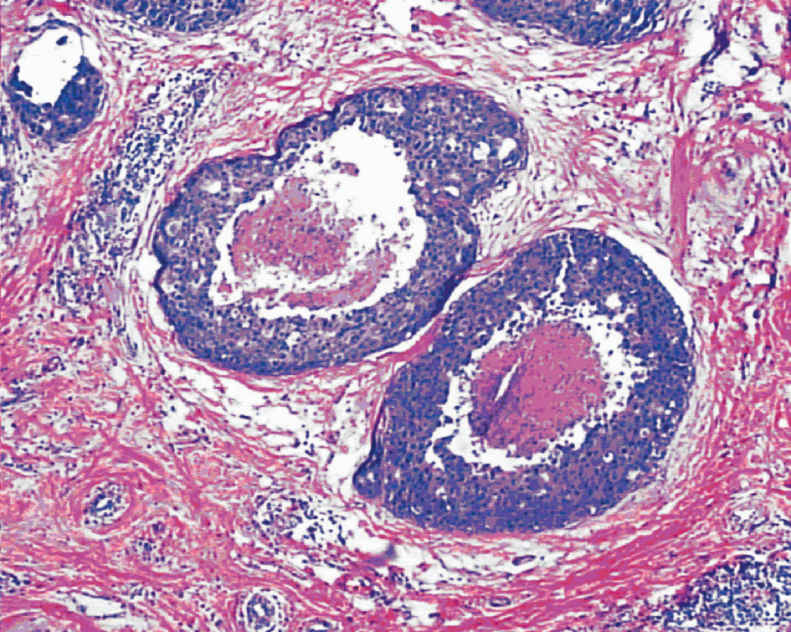
\includegraphics{./images/Image00202.jpg}
 \captionsetup{justification=centering}
 \caption{导管原位癌(HE染色,低倍)\\ {\small 导管内异型细胞增生,多层、实性,中央可见粉刺状坏死}}
\label{fig11-15}
  \end{figure}

\paragraph{小叶原位癌(lobular carcinoma in situ)}
起源于乳腺小叶终末导管。癌组织未穿破基底膜。临床检查时肿块不明显,常为活检时偶然发现。

肉眼观:肿块不明显,标本切面上见数毫米面积的乳腺组织隆起,呈淡红色,质软。

镜下观:低倍镜下依然可见小叶结构,小叶内终末导管即小叶单元扩大,上皮细胞增生充满扩张的末梢导管和腺泡,呈实性团巢。细胞体积大,形状大小一致,胞质量中等淡染,核大而圆,染色质细致,核分裂象罕见,一般无坏死,基底膜完整。

小叶原位癌一般发展缓慢,预后较好。

\subsubsection{浸润癌}

浸润性乳腺癌多由导管原位癌演变而来,少数来自小叶原位癌。肉眼观:肿瘤边界不清,质地坚硬,呈灰白色。切面如同果汁不多的梨肉,内有散在黄色小点,此为肿瘤坏死。晚期,肿瘤像树根样向周围浸润,深者可达筋膜,甚至浸润肌肉。

不同类型的浸润性乳腺癌在免疫表型上表现不同,雌激素受体(ER)、孕激素受体(PR)、原癌基因人类表皮生长因子受体2(HER2)和增殖活性指标Ki-67是目前乳腺癌的诊断、治疗和预后判断中最为常用的标记物,而免疫组织化学是最常用的检测方法。

病理组织学类型可分为下列几种:

\paragraph{浸润性导管癌}
非特指型(infiltrating ductal carcinoma,not
otherwise
specified),此型最常见,约占乳腺癌的75%。低倍镜下见随机排列的肿瘤细胞,缺乏肌上皮。管状成分可多可少,也可见梁索状或片状排列的癌细胞(图\ref{fig11-16})。癌细胞呈圆形或多角形,具有一定多形性和异型性,可见核分裂象及坏死。间质可从富于成纤维细胞(促结缔组织增生型)到大量胶原为主。伴有大量胶原性间质的癌,质地坚硬,癌细胞体积小、胞质少、核深染,且呈单行排列,散在分布,称为硬癌。硬癌浸润性强,高度恶性,预后差。

\begin{figure}[!htbp]
 \centering
 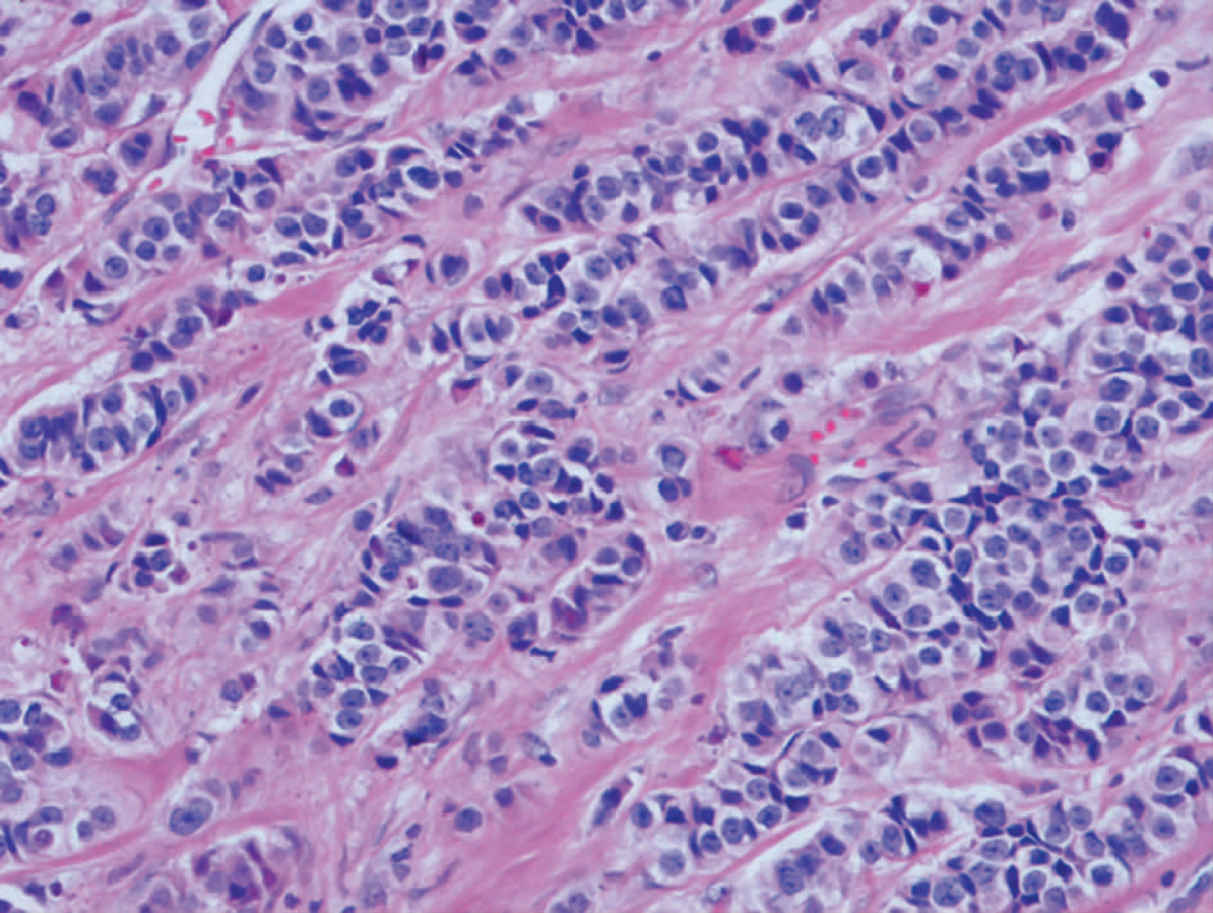
\includegraphics{./images/Image00203.jpg}
 \captionsetup{justification=centering}
 \caption{浸润性导管癌,非特指型(HE染色,高倍)\\ {\small 癌细胞呈梁索状或片状排列;圆形或多角形;间质主要为胶原纤维}}
\label{fig11-16}
  \end{figure}

\paragraph{浸润性小叶癌(invasive lobular carcinoma)}
占乳腺癌的5%~10%,小叶原位癌突破基底膜,浸润乳腺间质而来,常多中心性发生,而且双侧多见。肿块体积小,质硬,切面灰白色,部分病例病变可累及全乳。癌细胞缺乏黏附性,常呈单行排列,被纤维间质分隔。有时癌细胞围绕导管呈同心圆排列,似靶环状。经典的小叶癌癌细胞小而均一,异型性不明显,而多形性小叶癌瘤细胞则具有较大异型性。

浸润性小叶癌常表达ER、PR,较少表达HER2,一般不表达细胞黏附分子E-cadherin.鉴于本型肿瘤常可为双侧性,因此必须对另一侧乳腺加以仔细检查和随访。

\paragraph{特殊类型浸润癌}
(1)小管癌(tubular
carcinoma)少见,仅占乳腺癌的2%。临床常触不到,影像学上可表现为不规则肿块。一般瘤体较小。大体表现为境界不清的质硬肿块,切面常呈灰白色放射状浸润周围组织。镜下表现为无序排列的单层上皮小管浸润在纤维间质中,小管常形态不规则,成角或液滴状(图\ref{fig11-17})。免疫组化常表达ER、PR,一般不表达HER2,增殖指标Ki-67低表达。纯粹的乳腺小管癌(小管癌成分>90%)多为早期(I期)病变,较少发生腋窝淋巴结转移,预后好。

\begin{figure}[!htbp]
 \centering
 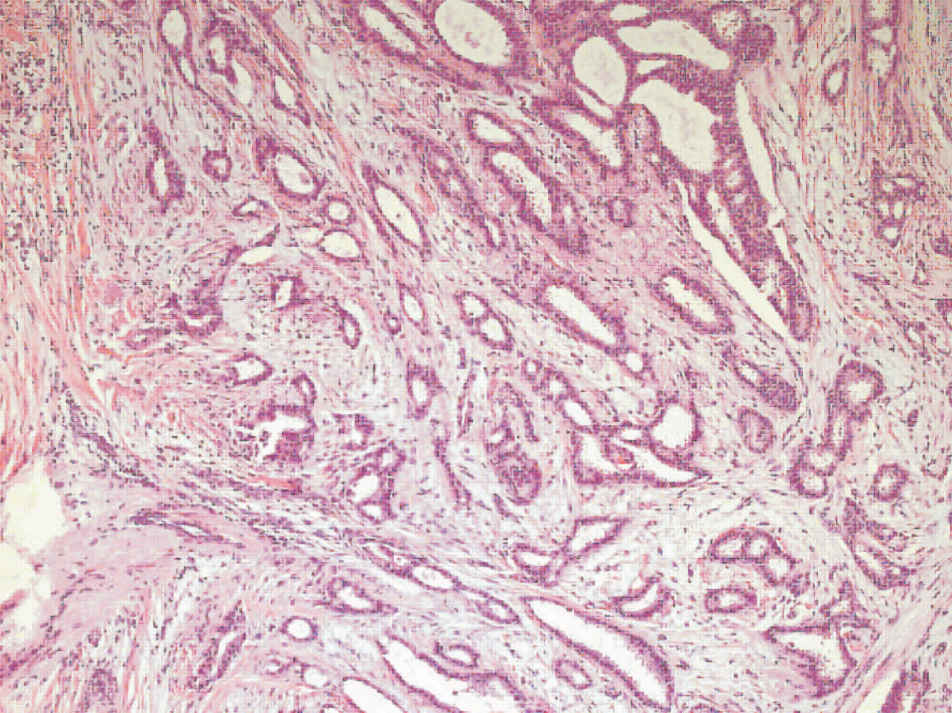
\includegraphics{./images/Image00204.jpg}
 \captionsetup{justification=centering}
 \caption{乳腺小管癌(HE染色,中倍)\\ {\small 瘤组织主要由单层排列的小管构成,小管形态不规则,无肌上皮}}
\label{fig11-17}
  \end{figure}

(2)髓样癌(medullary
carcinoma)少见,占乳腺癌的1%。临床表现与普通乳腺癌无明显差别,影像学上常表现为密度均匀一致的境界清楚的圆形、卵圆形或分叶状肿块,通常无钙化。大体表现上瘤体一般较大,质地较软。切面灰白色或灰红色境界清楚。镜下见癌细胞密集成片,合体状,高组织学级别核,核分裂多见。肿瘤间质少,显著的淋巴细胞和浆细胞浸润。免疫组化一般不表达ER、PR及HER2。此型肿瘤虽组织学形态呈高级别特点,但生长慢,很少发生转移,即使转移也限于腋窝下组淋巴结,故预后好。

(3)黏液癌(mucinous carcinoma)也称胶样癌(colloid
carcinoma)。纯粹的黏液癌(黏液癌成分>90%)甚少见,占乳腺癌的1%~2%。发病年龄大,好发于绝经后的妇女。临床通常表现为质地较软的肿块,影像学常表现为境界清楚或分叶状的结节。肉眼观:肿瘤界清,质地极软,切面呈灰白色、胶冻状。镜下观:大量细胞外黏液形成黏液湖,湖中漂浮着癌细胞岛。癌细胞簇状、索状或腺样排列,一般表达ER、PR,ER2通常不表达。本瘤生长慢,属低度恶性。

(4)乳头派杰氏病(Paget
disease)指乳腺导管内癌癌细胞沿导管蔓延至乳头和乳晕,在表皮层内可见典型的癌细胞(Paget
cell),占乳腺癌1%~3%。临床上常表现为乳头和乳晕皮肤粗糙不平,红肿、糜烂、渗液、结痂伴局部瘙痒和烧灼感,呈湿疹样改变,故又称湿疹样癌(eczematoid
carcinoma)。癌细胞体积大,胞质丰富淡染或透亮,核大而圆,核仁明显,核分裂象易见。其下方可以伴有或不伴有细胞形态相似的导管内癌成分,可伴间质浸润。通常ER、PR低表达,而HER2高表达。预后及治疗与其下方伴发的导管内癌或浸润性癌相关。

\subsubsection{乳腺癌的分子亚型}

乳腺癌是一种高度异质性的肿瘤。传统的乳腺癌分型以形态学为基础,这种分型与临床治疗和预后的相关性并不很强,有时会出现相同形态学亚型和组织学级别的乳腺癌对相同治疗的反应不同、预后迥异的情况,不能满足指导临床治疗、评估预后的需求。乳腺癌的分子分型以乳腺癌基因表达谱为依据,将乳腺癌分为腺腔A型(Luminal
A)、腺腔B型(Luminal B)、HER2过表达型(HER2-over
expression)、基底样型(Basal-like)。这种分型直接反映肿瘤在基因水平的异常,更接近肿瘤本质,与临床治疗和预后的关系也更为密切。由于基因表达谱分析尚不适于常规检测,因此目前通过免疫组织化学方法检测一组分子标志物的表达来替代基因表达谱分析,分型标准及相应治疗原则见表\ref{tab11-3}。

\begin{table}[ht]
    \caption{乳腺癌分子分型标准及相应治疗原则}
    \label{tab11-3}
    \centering
%    \begin{tabular}{lp{5cm}ll}
%    \toprule
%    分子亚型 & 分型标准 & 治疗策略\\
%    \midrule
 %   腺腔A & ER+/PR+/HER2-,且PR≥20\%,Ki-67<14\% & 单纯内分泌治疗\\
%腺腔B & 1. ER +/PR+/HER2-,而且Ki-67≥14\%和/或PR< 20\% & 内分泌治疗+/-细胞毒治疗\\
%HER2过表达型 & 2. ER+/PR +/HER2+ & 细胞毒治疗+内分泌治疗+抗HER2治疗\\
%&HER2过表达或扩增,ER-/PR-&细胞毒治疗+抗HER2治疗\\
%基底样型 & ER-/PR- /HER2-,CK5/6+和/或EGFR +&  细胞毒治疗\\
%    \bottomrule
 %   \end{tabular}
 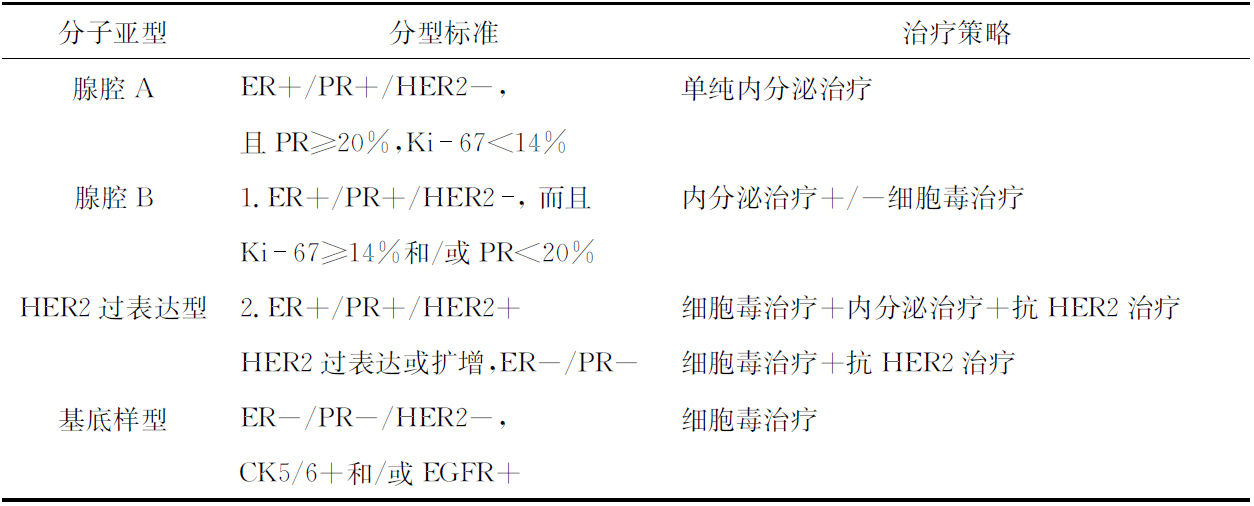
\includegraphics{./images/Image00205.jpg}
\end{table}

\subsection{扩散}

乳腺癌可直接蔓延破坏乳腺及胸壁组织,亦可发生淋巴道和血道转移。乳腺的淋巴液约75%回流至同侧腋窝淋巴结,是乳腺癌最常见的转移部位。晚期可转移到锁骨上、下内淋巴结,甚至胸骨旁及纵隔淋巴结,偶尔可转移到对侧腋窝淋巴结。乳腺癌血道转移以肺、骨、肝和肾上腺等为多见。

\subsection{结局}

乳腺癌的预后与其亚型和临床分期密切相关。腺腔A型一般预后较好,而HER2过表达型和大多数基底样型预后较差。肿瘤直径小于2
cm无淋巴结转移者,预后较好。若直径大于2
cm,有同侧腋窝淋巴结转移者预后相对较差,而直径大于5
cm伴有局部或远处转移者预后差。

\section{前列腺疾病}

\subsection{良性前列腺增生}

良性前列腺增生(benign prostatic
hyperp1asia,BPH)也称前列腺肥大,是老年男性的常见疾病,多发生于50岁以上的男性,发病率随年龄增加而升高。一般认为本病的病因与老年男性的睾丸萎缩导致的激素不平衡有关。

肉眼观:前列腺体积增大,重量增加,可达40 g以上(正常重约20
g),有时达200
g以上。若以腺体增生为主,则质地较软;切面常呈多结节状、乳白色,增生的腺管可扩张成大小不等的囊腺腔,类似海绵,挤压时囊内有乳白色分泌物流出。若以纤维组织和平滑肌增生为主,则质地较硬;切面可呈弥漫性增大而没有明显的结节形成。前列腺增生主要累及尿道周围的中叶,压迫尿道并常常突入膀胱,临床称之为前列腺中叶增生。

镜下观:增生的结节由增生程度不同的前列腺腺体、平滑肌和纤维组织组成(图\ref{fig11-18})。三种成分所占比例不同病例间可以不同,腺体和间质的比例也可有不同。增生的腺上皮有的呈高柱状,并呈乳头状突入腔内,胞质内有富含酸性磷酸酶的分泌颗粒;有的上皮为立方形,胞质内无分泌颗粒。增生的上皮均无异型性,上皮周围有基底细胞和完整的基膜围绕。腺腔中有红染的同心圆状凝聚物(淀粉样小体)。间质纤维、平滑肌组织肥大增生,包绕或穿插于增生的腺体之间,形成宽窄不一的间隔。此外,结节内可有小灶性坏死和淋巴细胞浸润。

\begin{figure}[!htbp]
 \centering
 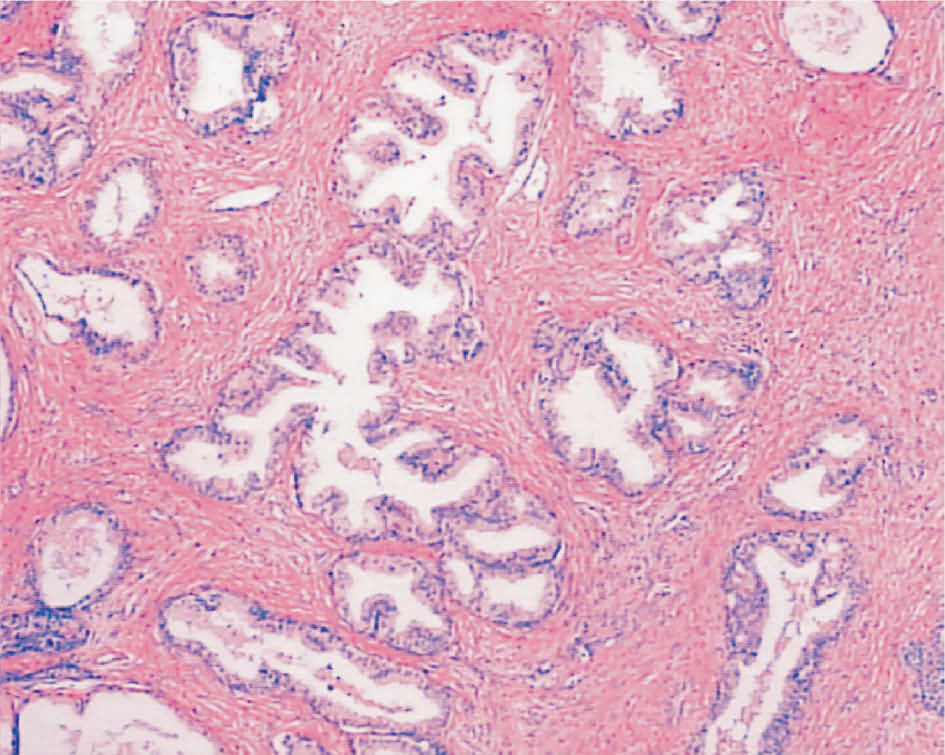
\includegraphics{./images/Image00206.jpg}
 \captionsetup{justification=centering}
 \caption{前列腺增生症(HE染色,低倍)\\ {\small 腺上皮呈乳头状增生伴间质平滑肌增生}}
\label{fig11-18}
  \end{figure}

前列腺增生主要发生于前列腺中央区和移行区,尿道前列腺部受压而表现为尿道阻塞症状。早期可出现尿频、滴尿、排尿困难等尿道梗阻症。随着病程进展,患者出现尿潴留、膀胱扩张和膀胱肌层肥厚等,重症者可发生肾盂积水,甚至肾衰竭。

\subsection{前列腺癌}

前列腺癌(carcinoma of
prostate)多发生于50岁以上的老年人。在欧美国家发生率较高,在美国前列腺癌占男性恶性肿瘤发病率的第一位,死亡率居第二位,本病在国内少见,近年有增高趋势。

前列腺癌病因尚不完全清楚。目前认为发生前列腺癌的危险因素有以下几点:①年龄:如前列腺癌常发生于50岁以上者。②种族:前列腺癌亚洲少见,而在欧美国家高发,尤其是美国黑人。美国黑人的发病率是白人的2倍,亚洲人的5倍。③遗传因素:研究证实,前列腺癌的发生和发展与人体一系列染色体的基因突变、缺失和染色体重排等分子遗传学密切相关。有家族史者前列腺癌的发病率比普通人群高3倍,在美国1/3的前列腺癌患者其遗传易感性研究定位于1q24-25。④激素水平:前列腺癌的发生与雄激素有关,原因是睾丸切除术和抑制雄激素治疗有效。⑤饮食因素:如摄入动物脂肪过多,其他如维生素C、维生素A和番茄红素缺乏等。

肉眼观:70%的前列腺癌发生于前列腺周围区,尤其是包膜下区多见,故临床上经肛门指检可触及肿块。肿瘤通常为多中心性,切面可见肿瘤呈黄白色,质地硬,境界不清。早期,肿瘤小,十分隐匿,称隐匿型前列腺癌。然而肿瘤虽然不大,却可早期广泛转移。晚期,肿瘤可扩展到全部前列腺,甚至穿破前列腺包膜,浸润精囊和膀胱底。

镜下观:97%的前列腺癌为腺癌,以高分化腺癌最多见,少数为鳞状细胞癌和移行细胞癌。通常,高分化的前列腺癌表现为形态较规则的小腺体,腺腔大小不等,排列紊乱,可见背靠背、腺体融合等现象。腺体由正常的两层上皮变为单层立方上皮或复层上皮,有时可呈乳头状生长,基底细胞消失。癌细胞具有不同程度的异型性。细胞核呈空泡状、核大深染、核仁明显。通常多形性不明显,核分裂不多见(图\ref{fig11-19})。分化较差的癌则可见较大的异型性,并可呈筛状、条索状、实性片状或单细胞分布。肿瘤间质为丰富的纤维结缔组织。此外,有时可见肿瘤侵犯血管、神经或前列腺包膜。

\begin{figure}[!htbp]
 \centering
 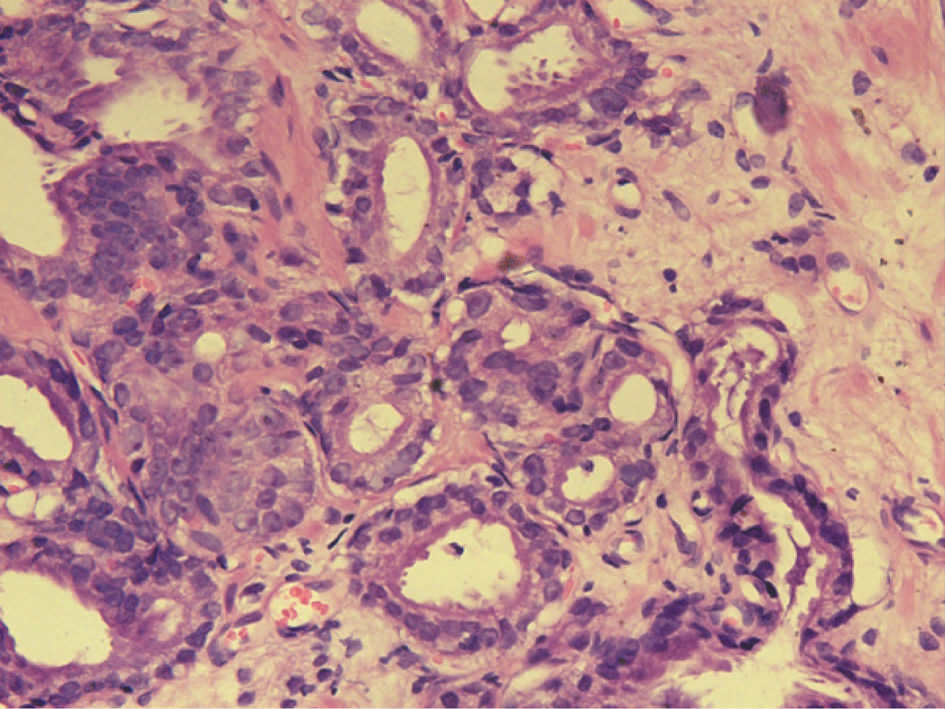
\includegraphics{./images/Image00207.jpg}
 \captionsetup{justification=centering}
 \caption{前列腺腺癌(HE染色,高倍)\\ {\small 高分化前列腺腺癌,异型小腺体,瘤细胞核大深染,核仁明显}}
\label{fig11-19}
  \end{figure}

前列腺癌可穿破包膜直接蔓延邻近器官,如膀胱、骶骨、精囊等。前列腺癌具有早期转移的特征,以血道及淋巴道转移为主。淋巴道转移最常见的是髂内、外动脉,腹主动脉旁等盆腔淋巴结和腹股沟淋巴结等。血道转移到骨、肺、肾上腺等处,尤其是腰椎、骨盆、肋骨的转移较常见。

免疫组织化学染色对前列腺癌的诊断有帮助。前列腺癌细胞可像正常前列腺组织一样分泌前列腺特异性抗原(prostatic
specific antigen,PSA)和酸性磷酸酶(prostatic acid
phosphatase,PAP),但恶性腺体缺乏基底细胞。因此大多数前列腺癌病例PSA和PAP均为阳性,而且基底细胞标记34βE12和p63阴性。这些指标在前列腺癌的诊断中起着重要作用,PSA和PAP还是临床上监测前列腺癌的重要指标。

\section*{复习与思考}

{一、名词解释}

子宫颈癌 CIN 宫颈早期浸润癌 水泡状胎块 恶性葡萄胎 粉刺癌 小叶原位癌 Paget病

{二、思考题}

1. 宫颈浸润癌的肉眼观类型有哪些?形态特点如何?

2. 试述宫颈鳞状细胞癌的发展过程及形态特征。

3. 试述宫颈癌的病理类型、蔓延和转移途径,有哪些严重后果?

4. 试从病理角度比较葡萄胎、恶性葡萄胎及绒毛膜癌的异同点。

5. 卵巢肿瘤按其组织发生可以分为哪三类?各举1例并简述其病理变化。

6. 乳腺癌患者乳腺外观可有哪些改变?是如何产生的?

7. 乳腺癌的常见组织学类型有哪些?

8. 乳腺癌的常见分子亚型有哪些?临床意义是什么?

9. 前列腺癌的常见临床表现是什么?

10. 前列腺癌病理及免疫组化诊断依据有哪些?